\documentclass{tufte-book}
\usepackage{amsmath}
\usepackage{amssymb}
\usepackage{array}
\usepackage[T1]{fontenc}
\usepackage[english, russian]{babel}

% For nicely typeset tabular material
\usepackage{booktabs}
\usepackage{cmap}
\usepackage{comment}
\hypersetup{colorlinks}% uncomment this line if you prefer colored hyperlinks (e.g., for onscreen viewing)
\usepackage{pscyr}

\usepackage[utf8]{inputenc}

\usepackage{indentfirst}

% For graphics / images
\usepackage{graphicx}
\setkeys{Gin}{width=\linewidth,totalheight=\textheight,keepaspectratio}
\graphicspath{{pictures/}}

\usepackage{floatrow}
\usepackage{textcomp}
\usepackage{multirow}
\usepackage{icomma}
\usepackage{enumitem}
\usepackage{verbatim}

% Prints a trailing space in a smart way.
\usepackage{xspace}

%%
% Book metadata
\title{Конструирование оптико-электронных приборов\thanks{Thanks to Edward R.~Tufte for his inspiration.}}
\author[Городничев В.А., Филимонов П.А.]{Городничев В.А., Филимонов П.А.}
\publisher{Кафедра РЛ-5 <<Элементы приборных устройств>> МГТУ им. Баумана}

%%
% If they're installed, use Bergamo and Chantilly from www.fontsite.com.
% They're clones of Bembo and Gill Sans, respectively.
%\IfFileExists{bergamo.sty}{\usepackage[osf]{bergamo}}{}% Bembo
%\IfFileExists{chantill.sty}{\usepackage{chantill}}{}% Gill Sans

%\usepackage{microtype}

%%
% Just some sample text
\usepackage{lipsum}

%%

% The fancyvrb package lets us customize the formatting of verbatim
% environments.  We use a slightly smaller font.
\usepackage{fancyvrb}
\fvset{fontsize=\normalsize}

%%
% Prints argument within hanging parentheses (i.e., parentheses that take
% up no horizontal space).  Useful in tabular environments.
\newcommand{\hangp}[1]{\makebox[0pt][r]{(}#1\makebox[0pt][l]{)}}

%%
% Prints an asterisk that takes up no horizontal space.
% Useful in tabular environments.
\newcommand{\hangstar}{\makebox[0pt][l]{*}}

%%


%%
% Some shortcuts for Tufte's book titles.  The lowercase commands will
% produce the initials of the book title in italics.  The all-caps commands
% will print out the full title of the book in italics.
\newcommand{\vdqi}{\textit{VDQI}\xspace}
\newcommand{\ei}{\textit{EI}\xspace}
\newcommand{\ve}{\textit{VE}\xspace}
\newcommand{\be}{\textit{BE}\xspace}
\newcommand{\VDQI}{\textit{The Visual Display of Quantitative Information}\xspace}
\newcommand{\EI}{\textit{Envisioning Information}\xspace}
\newcommand{\VE}{\textit{Visual Explanations}\xspace}
\newcommand{\BE}{\textit{Beautiful Evidence}\xspace}

\newcommand{\TL}{Tufte-\LaTeX\xspace}

% Prints the month name (e.g., January) and the year (e.g., 2008)
\newcommand{\monthyear}{%
  \ifcase\month\or January\or February\or March\or April\or May\or June\or
  July\or August\or September\or October\or November\or
  December\fi\space\number\year
}


% Prints an epigraph and speaker in sans serif, all-caps type.
\newcommand{\openepigraph}[2]{%
  %\sffamily\fontsize{14}{16}\selectfont
  \begin{fullwidth}
  \sffamily\large
  \begin{doublespace}
  \noindent\allcaps{#1}\\% epigraph
  \noindent\allcaps{#2}% author
  \end{doublespace}
  \end{fullwidth}
}

% Inserts a blank page
\newcommand{\blankpage}{\newpage\hbox{}\thispagestyle{empty}\newpage}

\usepackage{units}

% Typesets the font size, leading, and measure in the form of 10/12x26 pc.
\newcommand{\measure}[3]{#1/#2$\times$\unit[#3]{pc}}

% Macros for typesetting the documentation
\newcommand{\hlred}[1]{\textcolor{Maroon}{#1}}% prints in red
\newcommand{\hangleft}[1]{\makebox[0pt][r]{#1}}
\newcommand{\hairsp}{\hspace{1pt}}% hair space
\newcommand{\hquad}{\hskip0.5em\relax}% half quad space
\newcommand{\TODO}{\textcolor{red}{\bf TODO!}\xspace}
\newcommand{\ie}{\textit{i.\hairsp{}e.}\xspace}
\newcommand{\eg}{\textit{e.\hairsp{}g.}\xspace}
\newcommand{\na}{\quad--}% used in tables for N/A cells
\providecommand{\XeLaTeX}{X\lower.5ex\hbox{\kern-0.15em\reflectbox{E}}\kern-0.1em\LaTeX}
\newcommand{\tXeLaTeX}{\XeLaTeX\index{XeLaTeX@\protect\XeLaTeX}}
% \index{\texttt{\textbackslash xyz}@\hangleft{\texttt{\textbackslash}}\texttt{xyz}}
\newcommand{\tuftebs}{\symbol{'134}}% a backslash in tt type in OT1/T1
\newcommand{\doccmdnoindex}[2][]{\texttt{\tuftebs#2}}% command name -- adds backslash automatically (and doesn't add cmd to the index)
\newcommand{\doccmddef}[2][]{%
  \hlred{\texttt{\tuftebs#2}}\label{cmd:#2}%
  \ifthenelse{\isempty{#1}}%
    {% add the command to the index
      \index{#2 command@\protect\hangleft{\texttt{\tuftebs}}\texttt{#2}}% command name
    }%
    {% add the command and package to the index
      \index{#2 command@\protect\hangleft{\texttt{\tuftebs}}\texttt{#2} (\texttt{#1} package)}% command name
      \index{#1 package@\texttt{#1} package}\index{packages!#1@\texttt{#1}}% package name
    }%
}% command name -- adds backslash automatically
\newcommand{\doccmd}[2][]{%
  \texttt{\tuftebs#2}%
  \ifthenelse{\isempty{#1}}%
    {% add the command to the index
      \index{#2 command@\protect\hangleft{\texttt{\tuftebs}}\texttt{#2}}% command name
    }%
    {% add the command and package to the index
      \index{#2 command@\protect\hangleft{\texttt{\tuftebs}}\texttt{#2} (\texttt{#1} package)}% command name
      \index{#1 package@\texttt{#1} package}\index{packages!#1@\texttt{#1}}% package name
    }%
}% command name -- adds backslash automatically
\newcommand{\docopt}[1]{\ensuremath{\langle}\textrm{\textit{#1}}\ensuremath{\rangle}}% optional command argument
\newcommand{\docarg}[1]{\textrm{\textit{#1}}}% (required) command argument
\newenvironment{docspec}{\begin{quotation}\ttfamily\parskip0pt\parindent0pt\ignorespaces}{\end{quotation}}% command specification environment
\newcommand{\docenv}[1]{\texttt{#1}\index{#1 environment@\texttt{#1} environment}\index{environments!#1@\texttt{#1}}}% environment name
\newcommand{\docenvdef}[1]{\hlred{\texttt{#1}}\label{env:#1}\index{#1 environment@\texttt{#1} environment}\index{environments!#1@\texttt{#1}}}% environment name
\newcommand{\docpkg}[1]{\texttt{#1}\index{#1 package@\texttt{#1} package}\index{packages!#1@\texttt{#1}}}% package name
\newcommand{\doccls}[1]{\texttt{#1}}% document class name
\newcommand{\docclsopt}[1]{\texttt{#1}\index{#1 class option@\texttt{#1} class option}\index{class options!#1@\texttt{#1}}}% document class option name
\newcommand{\docclsoptdef}[1]{\hlred{\texttt{#1}}\label{clsopt:#1}\index{#1 class option@\texttt{#1} class option}\index{class options!#1@\texttt{#1}}}% document class option name defined
\newcommand{\docmsg}[2]{\bigskip\begin{fullwidth}\noindent\ttfamily#1\end{fullwidth}\medskip\par\noindent#2}
\newcommand{\docfilehook}[2]{\texttt{#1}\index{file hooks!#2}\index{#1@\texttt{#1}}}
\newcommand{\doccounter}[1]{\texttt{#1}\index{#1 counter@\texttt{#1} counter}}

% Generates the index
\usepackage{makeidx}
\makeindex

\begin{document}

% Front matter
\frontmatter

% r.3 full title page
\maketitle


% v.4 copyright page
\newpage
\begin{fullwidth}
~\vfill
\thispagestyle{empty}
\setlength{\parindent}{0pt}
\setlength{\parskip}{\baselineskip}
Copyright \copyright\ \the\year\ \thanklessauthor

\par\smallcaps{\thanklesspublisher}

\par\smallcaps{tufte-latex.googlecode.com}

\par Licensed under the Apache License, Version 2.0 (the ``License''); you may not
use this file except in compliance with the License. You may obtain a copy
of the License at \url{http://www.apache.org/licenses/LICENSE-2.0}. Unless
required by applicable law or agreed to in writing, software distributed
under the License is distributed on an \smallcaps{``AS IS'' BASIS, WITHOUT
WARRANTIES OR CONDITIONS OF ANY KIND}, either express or implied. See the
License for the specific language governing permissions and limitations
under the License.\index{license}

\par\textit{\monthyear}
\end{fullwidth}

% r.5 contents
\tableofcontents

\listoffigures

\listoftables

% r.7 dedication
\cleardoublepage
~\vfill
\begin{doublespace}
\noindent\fontsize{18}{22}\selectfont\itshape
\nohyphenation
Dedicated to those who appreciate \LaTeX{} 
and the work of \mbox{Edward R.~Tufte} 
and \mbox{Donald E.~Knuth}.
\end{doublespace}
\vfill
\vfill


% r.9 introduction
\cleardoublepage
\chapter*{Introduction}

This sample book discusses the design of Edward Tufte's
books\cite{Tufte2001,Tufte1990,Tufte1997,Tufte2006}
and the use of the \doccls{tufte-book} and \doccls{tufte-handout} document classes.


%%
% Start the main matter (normal chapters)
\mainmatter


\chapter{Оптико-электронные приборы}
\label{ch:tufte-design}

\newthought{Оптико-электронными приборами}\marginnote{\allcaps{ОПТИКО-ЭЛЕКТРОННЫЕ ПРИБОРЫ}} называются приборы, в которых информация об исследуемом или наблюдаемом объекте переносится оптическим излучением (содержится в оптическом сигнале), а ее первичная обработка сопровождается преобразованием этого излучения (оптического сигнала) в электрическую энергию (в электрический сигнал). 


В\marginnote{Далее может встречаться также термин <<оптические приборы>>, что будет подразумевать --- <<оптические приборы, содержащие в своем составе механические, электронные и оптические функциональные устройства и элементы>>, т.е. фактически --- ОЭП.} состав этих приборов входят как оптические, так и электронные звенья, причем и те и другие выполняют основные функции данного прибора, а не являются вспомогательными устройствами (например, узлами подсветки отсчетных шкал, устройствами термостабилизации).

ОЭП является сложной системой, включающей в себя большое число различных по своей физической природе и принципу действия звеньев -- аналоговых и цифровых преобразователей электрических сигналов, микропроцессоров, оптических, механических и электромагнитных узлов и др. Поэтому ОЭП часто называют оптико-электронными системами (ОЭС). 

Учитывая большое разнообразие ОЭП и их широкое применение в самых различных областях науки и техники  в курсе лекций рассмотрены общие для большинства ОЭП вопросы проектирования, достаточно общие и часто используемые на практике методы расчета и выбора основных параметров ОЭП, особенности конструкции и методы расчета параметров типовых узлов ОЭП.

Помимо исследуемого объекта (<<полезный>> излучатель) на рис.~\ref{pic:1OEPscheme} показаны и возможные на практике <<вредные>> излучатели (фоны, помехи). Взаимное расположение звеньев может быть и несколько иным. Отдельные звенья на практике представляют собой весьма сложные устройства, например, в состав источника излучения могут входить передающая оптическая система, фильтры, модулятор. Иногда в состав ОЭП не входят некоторые из перечисленных звеньев. Это определяется, как правило, методом работы прибора.

Все ОЭП предназначены для получения информации об объектах окружающей среды, переносимой оптическими сигналами. Хорошо известны ОЭП, используемые для локации, исследования природных ресурсов, измерения оптических свойств различных объектов. Многие ОЭП работают в составе следящих систем, используемых в навигации и ориентации, в системах технического зрения, устройствах автоматического контроля и управления, системах управления летательными аппаратами, системах наведения и во многих других устройствах для измерения линейных, угловых величин и определения координат объектов. Определенной спецификой обладают оптико-электронные системы противодействия и подавления оптических схем противника.

\begin{figure}[h]
	\includegraphics[width=\linewidth]{1OEPscheme.png}%
	\caption{Обобщенная схема ОЭП}%
	\label{pic:1OEPscheme}%
\end{figure}

Главный элемент --- оптическая система (ее сложно разработать, обеспечить нужное качество), которая определяется оптической схемой. С оптической схемы начинается разработка ОЭП.

\textsc{Оптической схемой}\marginnote{\allcaps{ОПТИЧЕСКАЯ СХЕМА}} называется графическое представление процесса изменения света в оптической системе.

Различия в принципах работы звеньев ОЭП, в способах обработки сигналов, проходящих через них, а также разнообразие условий эксплуатации ОЭП обусловливают сложность и многоступенчатость процесса проектирования этих приборов и требуют тщательного анализа как условий работы ОЭП, так и состояния имеющейся в распоряжении разработчика элементной базы.

\section{Классификация ОЭП}

Классификация ОЭП возможна по широкому кругу признаков в зависимости от принципов построения приборов и характера их применения (рис.~\ref{pic:1Classification}). К числу таких признаков могут быть отнесены параметры оптического сигнала, метод измерений, спектральный диапазон работы, режим работы, степень автоматизации, вид измерений, назначение и область применения, условия эксплуатации.

\begin{figure*}[h]
	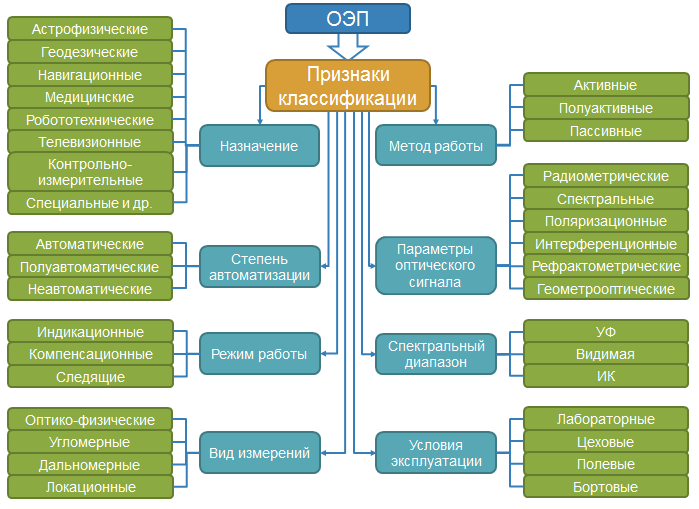
\includegraphics[width=\linewidth]{1classification.png}
	\caption{Обобщенная схема ОЭП}%
	\label{pic:1Classification}%
\end{figure*}

Как известно, в ОЭП носителем полезной информации служит оптический сигнал в виде потока излучения, являющийся функцией координат $(x, y, z)$ измеряемого объекта, спектрального состава излучения ($\lambda$), времени ($t$), состояния и положения плоскости поляризации излучения ($A_\text{п}$), т.е. $\Phi(x, y, z, \lambda, t, A_\text{п})$. 

По методу работы ОЭП с учетом особенностей их построения и возможности управления параметрами излучения ОЭП делят на:
\begin{itemize}
	\item активные (наблюдаемый объект освещается (с помощью передающей оптической системы) лазером, при этом часть отраженного излучения поступает на вход ОЭП);
	\item полуактивные (один источник освещает все объекты);
	\item пассивные (используется собственное излучение исследуемого объекта; тепловое  (отраженное) от других источников излучения (солнца, луны); рассеянное излучение атмосферы и подстилающей поверхности).
\end{itemize}

В зависимости от спектрального состава используемого излучения ОЭП подразделяют на приборы, работающие в следующих областях спектра:
\begin{enumerate}
	\item ультрафиолетовая (УФ)~--- 200--380~нм ;
	\item видимая --- 400--700~нм;
	\item инфракрасная (ИК) --- 700 нм--1~мм.
\end{enumerate}

В свою очередь, УФ делится на: УФ-А (400--315 нм), УФ-Б (315--280 нм), УФ-С: (280--10 нм). Излучение с длиной волны менее 200 нм называют вакуумным ультрафиолетом, так как излучение не распространяется из-за полного поглощения в атмосфере.

ИК диапазон условно разделяют на: ИК-А или ближний ИК (700--1400 нм), ИК-Б или средний ИК (1400--3000 нм), ИК-С или дальний ИК (3 мкм--1 мм).

По степени автоматизации различают ОЭП:
\begin{enumerate}
	\item автоматические, работающие без участия оператора (обычно в следящем режиме);
	\item полуавтоматические, функционирование которых частично зависит от действий оператора;
	\item неавтоматические, выходная информация которых рассчитана на восприятие оператором.
\end{enumerate}

Существенные различия в принципах построения, функционирования и обслуживания имеют ОЭП, работающие в различных условиях эксплуатации:
\begin{enumerate}
	\item лабораторные;
	\item цеховые;
	\item полевые;
	\item бортовые.
\end{enumerate}

Наиболее емким из приведенных признаков классификации является назначение (область применения). Практически невозможно найти область техники, где бы в настоящее время не применялись ОЭП. Поэтому в схеме классификации указаны только некоторые области техники, в которых применение ОЭП является решающим фактором их дальнейшего развития: 
\begin{enumerate}
	\item навигация (гирометры);
	\item геодезия (теодолит);
	\item астрофизика (телескопы);
	\item робототехника (система машинного зрения);
	\item телевизионная техника (подсветка и формирование изображения);
	\item медицина (микроскопы);
	\item контрольно-измерительная техника (интерферометры);
	\item военная техника (оптические прицелы).
\end{enumerate}

ОЭП внутри каждой из рассмотренных классификационных групп могут подразделяться по конструктивным, функциональным и иным признакам. Кроме того, между всеми классификационными признаками существуют прямые и косвенные связи. Например, контрольно-измерительные приборы могут быть угломерными, автоматическими, цеховыми.

\section{Основные критерии оценки качества ОЭП}

\newthought{Качеством прибора}\marginnote{\allcaps{КАЧЕСТВО ПРИБОРА}} называется совокупность свойств прибора, обуславливающих его пригодность удовлетворять определенные потребности в соответствии с его назначением. Для объективной оценки качества прибора его свойства характеризуют количественно~--- показателями качества.

\textsc{Показатели качества}\marginnote{\allcaps{ПОКАЗАТЕЛИ КАЧЕСТВА}}~--- это комплекс показателей, используемых для оценки свойств прибора, а также решений, принимаемых на различных этапах проектирования. Вследствие специфики ОЭП и разнообразия условий их производства оценка качества связана с рассмотрением широкого круга показателей, представленных на рис.~\ref{pic:1QualityOEP}.


Всесторонняя оценка современных изделий может быть выполнена лишь при комплексном учете всех указанных показателей. Вместе с тем при проектировании разработчики чаще всего оценивают качество будущего прибора по показателям функционирования, надежности и технологичности.

\newthought{Показатели функционирования}\marginnote{\allcaps{ПОКАЗАТЕЛИ ФУНКЦИОНИРОВАНИЯ}} являются основными, они характеризуют техническую сущность прибора, и именно поэтому они стоят на первом месте в техническом задании.

Ввиду большого разнообразия ОЭП показатели функционирования могут быть самыми различными. Достаточно обобщенными являются информационные характеристики, к которым относят:
\begin{enumerate}
	\item входной язык, посредством которого осуществляется связь прибора с наблюдаемым или контролируемым объектом;
	\item энергия, необходимая для формирования единицы информации;
	\item функция преобразования, описывающая зависимость информативного параметра выходного сигнала от информативного параметра входного сигнала при номинальных значениях неинформативных параметров;
	\item выходной язык, посредством которого осуществляется связь прибора с потребителем информации;
	\item скорость выдачи информации прибором и восприятия ее потребителем (быстродействие).
\end{enumerate}

Наряду с перечисленными к показателям функционирования могут быть отнесены также вид потребляемой энергии и мощность потребления, габаритные размеры и масса прибора.

\newthought{Надёжность}\marginnote{\allcaps{НАДЁЖНОСТЬ}} определяется как свойство объекта сохранять во времени в установленных пределах значения всех параметров, характеризующих способность выполнить требуемые функции в заданных режимах и условиях применения, технического обслуживания, ремонта, хранения и транспортирования.

Сложность ОЭП, включающих оптические, механические и электронные узлы, требования к работоспособности этих приборов в резко изменяющихся условиях эксплуатации ставят перед конструктором задачу~--- создать прибор, обладающий высокой надежностью в течение всего срока службы.

Надёжность прибора зависит от количества и качества входящих в него элементов, условий работы (температуры, влажности, механических воздействий), схемного и конструктивного выполнения прибора, технологии изготовления и качества материала элементов.

\newthought{Технологичность}\marginnote{\allcaps{ПОКАЗАТЕЛИ ТЕХНОЛОГИЧНОСТИ}} деталей, узлов и конструкций, удобство сборки может быть охарактеризована следующими показателями: 
\begin{itemize}
	\item минимальными затратами труда на изготовление;
	\item минимальным ассортиментом средств изготовления;
	\item минимумом сложных и трудоемких производственных процессов;
	\item простотой подготовки производства;
	\item минимальным числом операций и временем их проведения;
	\item правильным выбором допусков на изготовление;
	\item простота монтажа деталей в узлы без дополнительной обработки;
	\item законченность узлов, входящих в прибор;
	\item простота сборки прибора в целом.
\end{itemize}

\textsc{Рациональный выбор материалов}: материалы, необходимые для изготовления деталей, следует выбирать с учетом не только функциональных и эксплуатационных особенностей прибора, но и технологии его изготовления. Для единичного производства целесообразно использовать материалы, хорошо поддающиеся обработке резанием. При крупносерийном и массовом производстве более экономичны способы изготовления без снятия стружки, что и определяет в значительной степени выбор материалов.

\textsc{Минимальная номенклатура элементов, материалов, полуфабрикатов} упрощает снабжение производства. 
Кроме того, необходимо иметь в виду, что некоторые детали и элементы часто не соответствуют специфике и профилю предприятия. В этих случаях целесообразнее идти по пути кооперации с другими предприятиями, чем осваивать производство соответствующих изделий.

\textsc{Обеспечение взаимозаменяемости деталей, узлов и блоков} предполагает идентичность конструктивных и присоединительных размеров, соединителей, а также входных и выходных параметров. Взаимозаменяемость позволяет обеспечить замену одного узла или блока другим без дополнительной подгонки и регулирования. Это обстоятельство имеет важное значение при сборке приборов, особенно при крупносерийном и массовом производстве, а также при обслуживании и ремонте приборов. Прежде всего необходимо стремиться к взаимозаменяемости электронных узлов и блоков. Взаимозаменяемость обеспечивается рациональными допусками на размеры и параметры узлов и блоков.

\textsc{Максимальная нормализация и унификация конструкций} основана на применении нормализованных, унифицированных или стандартизованных деталей и узлов. Нормализованные детали включены в нормаль данного предприятия или группы родственных предприятий. Унифицированные детали применяются на предприятиях всей отрасли промышленности. Стандартизованные детали используются на предприятиях различных отраслей промышленности.

Унифицированные и стандартизованные детали, узлы и блоки изготовляются централизованно, что позволяет автоматизировать процесс их производства, обеспечить высокую надежность и минимальную стоимость. Показатели унификации и стандартизации характеризуют степень использования и применения в данном приборе стандартизованных, унифицированных и заимствованных узлов и деталей. Чем больше таких элементов будет в проектируемом приборе, тем меньше затраты на их конструирование, технологическую подготовку производства, выше, как правило, надежность функционирования, проще организовать обслуживание и ремонт.

\textsc{Обеспечение возможности изготовления деталей при единичном и мелкосерийном производстве на универсальном оборудовании} имеет смысл при изготовлении уникальных и экспериментальных приборов, для выпуска которых в единичных образцах или малыми сериями нецелесообразно делать специальную технологическую оснастку. Повысить качество таких приборов и уменьшить технологические и трудовые затраты на их изготовление можно путем использования типовых узлов и деталей, о которых говорилось выше.

\textsc{Простота и удобство выполнения сборки, монтажа и юстировки} имеет особое значение для качественной настройки прибора, как в заводских условиях, так и в процессе дальнейшего использования. При этом снижаются трудовые затраты и требования к уровню подготовки производственного и обслуживающего персонала, а также требования к сложности юстировочного и стендового оборудования.

\newthought{Эстетические показатели}\marginnote{\allcaps{ЭСТЕТИЧЕСКИЕ ПОКАЗАТЕЛИ}} характеризуют внешний вид прибора, его соответствие современному стилю, гармоничность сочетания отдельных элементов прибора друг с другом, соответствие формы прибора его назначению, качество и совершенство отделки внешних элементов, поверхностей и упаковки, выразительность и качество надписей, знаков, технической документации (проспекта, каталога, инструкции, паспорта).

\newthought{Патентно-правовые показатели}\marginnote{\allcaps{ПАТЕНТНО-ПРАВОВЫЕ ПОКАЗАТЕЛИ}} характеризуют степень новизны заложенных в ОЭП технических решений а также вопросы патентно-правовой  защиты и определяются патентоспособностью и патентной чистотой. Патентоспособным является решение, которое может быть признано изобретением в одной или нескольких странах. Патентной чистотой обладают решения, не попадающие под действие (не нарушающие прав) других патентов.

\newthought{Показатели техники безопасности}\marginnote{\allcaps{ПОКАЗАТЕЛИ ТЕХНИКИ БЕЗОПАСНОСТИ}} характеризуют степень защищенности людей и животных от опасного воздействия ОЭП (защита от электрического удара, электромагнитных полей, теплового воздействия, радиации, оптических излучений, шума, токсичных и газовых выделений, вибраций), а также самих приборов от климатических, механических, биологических и других воздействий на них. Такими показателями, например, являются категория и класс исполнения и эксплуатации.

\newthought{Экономические показатели}\marginnote{\allcaps{ЭКОНОМИЧЕСКИЕ ПОКАЗАТЕЛИ}} выражаются прежде всего в стоимости прибора. К основным факторам, определяющим стоимость прибора, относятся область применения, условия эксплуатации, технологичность конструкции, требования по надежности, серийность выпуска, стоимость материалов и комплектующих изделий, простота и удобство обслуживания, юстировок и ремонта. 

Экономические показатели характеризуют уровень затрат на производство и эксплуатацию ОЭП. Среди них выделяют полную себестоимость и оптовую цену прибора. 

\newthought{Эргономические показатели}\marginnote{\allcaps{ЭРГОНОМИЧЕСКИЕ ПОКАЗАТЕЛИ}} характеризуют степень приспособленности прибора к взаимодействию с человеком с позиции удобства работы, гигиены, безопасности труда. 

Эргономические показатели разделены на гигиенические (уровень шума, амплитуда и частота вибраций, уровень радиации, температура, степень загазованности, токсичности), антропометрические (размеры и расположение экранов, индикаторов, рукояток, наглазников, налобников, форма сиденья), психофизиологические (диапазоны усилий на рукоятках, скорость выполнения движений, уровень освещенности, цвет и яркость световых сигналов, тембр и сила звуковых сигналов), психологические (объем и интенсивность потока информации, количество и частота выполняемых операций, количество и расположение контрольных, сигнальных, управляемых элементов).

\newthought{Экологические показатели}\marginnote{\allcaps{ЭКОЛОГИЧЕСКИЕ ПОКАЗАТЕЛИ}} характеризуют степень вредного влияния на окружающую среду и ее загрязнение при изготовлении, эксплуатации и утилизации приборов.

\newthought{Передаточные системы ОЭП} выделяются по виду преобразуемого сигнала: механическая, оптическая и электронная.

\chapter{Зубчатые элементарные передачи}
\label{ch:gears}

\newthought{Механическая система ОЭП} выполняет функцию позиционирования различных элементов оптической системы в пространстве с заданной точностью.
Вид движения оптических элементов зависит от их назначения, но в большинстве случаев можно выделить вращательное и поступательное движения.
Передача энергии в механической системе ОЭП осуществляется различными механизмами.

\noindent
\textsc{Механизм}\marginnote{\allcaps{МЕХАНИЗМ}} --- система тел, предназначенная для преобразования движения одного или нескольких твердых тел в требуемое движение других твердых тел.

\noindent
\textsc{Кинематическая пара}\marginnote{\allcaps{КИНЕМАТИЧЕСКАЯ ПАРА}} --- соединение двух соприкасающихся звеньев, допускающих их относительное движение.

\noindent
\textsc{Кинематическая цепь}\marginnote{\allcaps{КИНЕМАТИЧЕСКАЯ ЦЕПЬ}} --- система звеньев, связанных между собой кинематическими парами.

\noindent
\textsc{Зубчатая элементарная передача}\marginnote{\allcaps{ЗУБЧАТАЯ ЭЛЕМЕНТАРНАЯ ПЕРЕДАЧА}} --- механизм, состоящий из зубчатых колёс, назначение которого --- передача вращательного движения между валами, обычно с изменением скоростей вращения или направления и характера движения.

Классификация передач осуществляется по различным признакам, основные из которых:
\begin{itemize}
	\item передаточное отношение: постоянное или переменное;
	\item характер движения: меняет или не меняет направление;
	\item взаимное расположение осей: параллельное, пересекающиеся и скрещивающиеся;
	\item характер изменения скорости (замедление или ускорение);
	\item вид зубьев колес: прямозубые, косозубые, с внешним или внутренним зацеплением.
\end{itemize}

Механизмы характеризуются следующими параметрами:
\begin{itemize}
	\item кинематические параметры: функция положения $ y = f(x_i, q_s) $, передаточное отношение $ i $;
	\item точностные -- погрешности перемещения, положения и передаточного отношения;
	\item технологические;
	\item конструктивные.
\end{itemize}

\newthought{Основная теорема зацепления}\marginnote{\allcaps{ОСНОВНАЯ ТЕОРЕМА ЗАЦЕПЛЕНИЯ}}: общая нормаль к профилям зубьев колес, проведенная через точку касания профилей, делит межосевое расстояние колес на отрезки, пропорциональные угловым скоростям вращения.

Известна угловая скорость $ \omega_1 $ зубчатого колеса 1, а следовательно, и окружные скорости точек профиля его зуба, в том числе и точки $ K $ касания профилей зубьев, $ v_{1K} = \omega_1 O_1 K $. Для точки $ K $ профиля зуба ведомого колеса известно направление окружной скорости $ v_{2K} $, оно перпендикулярно радиусу $ O_2 K $. Из очевидного условия, что проекции скоростей соприкасающихся точек $ K $ профилей зубьев колёс 1 и 2 на общую нормаль $ n-n $ должны быть одинаковы, т.е. $ v_{1n} = v_{2n}$, получаем:
\begin{equation*}
\omega_1 O_1 N_1 = \omega_2 O_2 N_2, \text{или}\, i=\dfrac{\omega_1}{\omega_2} = \dfrac{O_2 N_2}{O_1 N_1}.
\end{equation*}

Так как $ \triangle O_1 N_1 P \propto O_2 N_2 P $, то $ \dfrac{O_2 N_2}{O_1 N_1} = \dfrac{O_2 P}{O_1 P}$. Отсюда следует, что
\begin{equation*}
i=\dfrac{\omega_1}{\omega_2} = \dfrac{O_2 N_2 }{O_1 N_1} = \dfrac{O_2 P}{O_1 P}.
\end{equation*}

Для получения постоянного передаточного отношения на всём участке зацепления зубьев необходимо, чтобы $ i=\dfrac{\omega_1}{\omega_2} = \dfrac{O_2 P}{O_1 P} = const $. Таким образом, при передаче зацеплением общая нормаль к профилям зубьев в любой точке их касания при повороте колёс должна проходить через одну и ту же точку $ P $, которая делит межосевое расстояние $ a_w $ на отрезки, обратное отношение которых $ \dfrac{O_2 P}{O_1 P} $ равно передаточному отношению $ i=\dfrac{\omega_1}{\omega_2} $. Профили зубьев колёс передачи называют сопряжёнными, если они соответствуют основной теореме зацепления.

Определённым\marginnote{\allcaps{СКОЛЬЖЕНИЕ ПРОФИЛЕЙ}} недостатком зубчатых зацеплений является \allcaps{скольжение профилей зубьев}. Скорость скольжения $ v_\text{ск} $ профилей зубьев равна разности проекций скоростей контактирующих точек зубьев на направление касательной $ t-t $ к профилям в точке их касания: 
\begin{equation}
\label{eq:gears_skolzhenie}
v_\text{ск}=v_{1t} - v_{2t} = -PK (\omega_1 + \omega_2).
\end{equation}

Из выражения \ref{eq:gears_skolzhenie} следует, что чем дальше от полюса P происходит контакт профилей зубьев, тем больше скольжение профилей.
Скольжение профилей отсутствует, когда точка их касания находится в полюсе P. Полюс P является также мгновенным центром качения начальных окружностей, которые всегда касаются в полюсе. Это окружности диаметров $ d_{w1}, \, d_{w2} $. Таким образом:
\begin{equation*}
i=\dfrac{O_2 P}{O_1 P} = \dfrac{d_{w2}}{d_{w1}}.
\end{equation*}

\noindent
Следовательно, сопряжённые профили воспроизводят такую же передачу движения, как и исходные начальные окружности при их относительном качении без проскальзывания.

\textsc{Эвольвента}\marginnote{\allcaps{ЭВОЛЬВЕНТА}} --- кривая, представляющая собой траекторию движения любой точки прямой, перекатывающейся без скольжения по окружности.

\begin{table}[ht]
	\centering
	\fontfamily{ppl}\selectfont
	\begin{tabular}{ll}
		\toprule
		Обозначение & Параметр \\ 
		\midrule
		$ m $ & модуль зацепления, [мм] \\
		$ z_1,\,z_2 $ & количество зубьев \\
		$ d_1,\,d_2 $ & диаметр делительной окружности, [мм] \\
		$ p=s+e $ & шаг зубьев, [мм] \\
		$ s $ & толщина зубьев, [мм] \\
		$ e $ & расстояние между профилями зубьев, [мм] \\
		$ d_a $ & диаметр окружности впадин, [мм] \\
		$ d_a $ & диаметр окружности вершин, [мм] \\
		$ h $ & высота зуба, [мм] \\
		$ h_f $ & высота головки зуба, [мм] \\
		$ \tau $ & центральный угол делительной окружности \\
		$ b $ & наименьшее расстояние между торцами зубьев \\
		\bottomrule
	\end{tabular}
	\caption{Основные параметры зубчатого колеса}
	\label{tab:parZ}
\end{table}


\newthought{Достоинства} прямозубой передачи:
\begin{itemize}
	\item высокое передаточное отношение (до 15);
	\item надежность и простота обслуживания;
	\item технологичность;
	\item малые габариты;
	\item высокий КПД (до 0,99);
	\item постоянство передаточного отношения $ i $;
	\item применение в широком диапазоне вращающих моментов, скоростей и передаточных отношений;
	\item малые нагрузки на валы и опоры;
	\item долговечность (до 50000 ч).
\end{itemize}

\newthought{Недостатки} прямозубой передачи:
\begin{itemize}
	\item высокие требования к точ­ности изготовления и монтажа и, как следствие, дороговизна;
	\item шум при работе со значительными скоростями;
	\item высокая жесткость, не позволяющая компенсировать динамические нагрузки;
	\item невозможность безступенчатого регулирования передаточного отношения.
\end{itemize}

\begin{flushleft}
	\textbf{Моменты в передаче}
\end{flushleft}


\begin{flushleft}
	\textbf{Силовые соотношения}
\end{flushleft}

\begin{flushleft}
	\textbf{КПД}
\end{flushleft}


\begin{flushleft}
	\textbf{Минимальное число зубьев}
\end{flushleft}

\textsc{Методы нарезания зубьев}\marginnote{\allcaps{МЕТОДЫ НАРЕЗАНИЯ ЗУБЬЕВ}}:
\begin{itemize}
	\item метод деления (копирования);
	\item метод обката (огибания).
\end{itemize}

Для\marginnote{\allcaps{КОРРИГИРОВАННЫЕ ЗУБЧАТЫЕ ПЕРЕДАЧИ}} устранения подрезания зубьев применяют \textsc{корригированные зубчатые передачи}.
Корригирование определяется смещением режущего инструмента $ x = \xi m $ при нарезании зубьев:
\begin{itemize}
	\item отсутствие коррекции (нулевая передача): $ \xi_1 = \xi_2 = 0, \, \xi_\Sigma=0 $;
	\item высотная коррекция (равносмещённая передача): $ \xi_1 = -\xi_2 \neq 0, \, \xi_\Sigma=0 $;
	\item угловая коррекция, при которой происходит изменение угла зацепления: $ \xi_1 \neq \xi_2, \, \xi_\Sigma \neq 0 $, различают положительные ($\xi_\Sigma > 0 $) и отрицательные ($\xi_\Sigma < 0 $) передачи.
\end{itemize}

\marginnote{\allcaps{КОРРИГИРОВАННЫЕ ЗУБЧАТЫЕ ПЕРЕДАЧИ}}
\begin{flushleft}
	\textbf{Материалы прямозубых и косозубых цилиндрических зубчатых колёс}
\end{flushleft}


\section{Точность зубчатых колёс и передач}

\newthought{Точные приборные устройства}\marginnote{\allcaps{ТОЧНЫЕ ПРИБОРНЫЕ УСТРОЙСТВА}}~--- приборные устройства, точность работы которых регламентируется допусками.\marginnote{Допуск на точность обозначается $ [\delta_0 S] $}

Расчеты на точность подразделяются на:
\begin{itemize}
	\item прямой (проектный) -- определение точностных требований к составляющим устройствам, узлам и деталям;
	\item обратный (проверочный) -- определение погрешности ПУ на основе разработанных точностных требований к звеньям устройства.
\end{itemize}

Существует 12 степеней точности. В приборостроении обычно применяют 6-9 степени точности.

\newthought{Показатели точности} регулируются стандартами (контрольные комплексы):
\begin{itemize}
	\item \allcaps{кинематическая точность}\marginnote{\allcaps{КИНЕМАТИЧЕСКАЯ ТОЧНОСТЬ}} --- наибольшая погрешность функции положения при работе передачи в одном направлении или наибольшая погрешность $ i $;
	\item \allcaps{плавность работы}\marginnote{\allcaps{ПЛАВНОСТЬ РАБОТЫ}} --- плавность изменения кинематической погрешности – колебания скорости за один оборот, источник динамической нагрузки;
	\item \allcaps{пятно контакта}\marginnote{\allcaps{ПЯТНО КОНТАКТА}} --- полнота прилегания зубьев и концентрация нагрузки на их поверхности;
	\item \allcaps{боковой зазор}\marginnote{\allcaps{БОКОВОЙ ЗАЗОР}} между работающими профилями зубев --- для компенсации температурных деформаций, смазки, погрешностей сборки и изготовления; боковой зазор нормируется независимо от степени точности зубчатых колёс и передач, определение которого основано на величине минимального гарантированного бокового зазора $ j_{n\,min} $.
\end{itemize}

Для всех видов передач предпочтительными являются функциональные показатели  и суммарное пятно контакта.

\section{Проектный расчёт зубчатых передач на прочность}
\textsc{Выкрашивание}\marginnote{\allcaps{ВИДЫ РАЗРУШЕНИЙ ЗУБЧАТЫХ КОЛЁС}} поверхностных слоев зубьев характерно для закрытых хорошо смазываемых передач. При циклическом нагружении на поверхности зубьев у полюсной линии разрастаются микротрещины, что приводит к образованию оспинок, переходящих в раковины. Выкрашивание может быть ограниченным или прогрессирующим.

\textsc{Поломка зубьев} может носить усталостный характер или являться следствием значительных перегрузок. При циклическом нагружении микротрещины у корня зуба разрастаются, что приводит к излому по сечению у основания зуба прямозубых колёс или по косому сечению – косозубых и шевронных колёс.
\begin{marginfigure}
	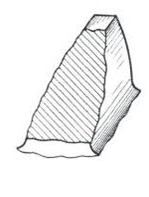
\includegraphics[width=0.4\linewidth]{polomkaZ.png}
\end{marginfigure}

\textsc{Абразивный износ} характерен для открытых передач, а также закрытых, работающих при скудной смазке и наличии абразивов.

\textsc{Заедание} характерно для высоконагруженных передач. При высокой удельной нагрузке происходит разрыв масляной плёнки, нагрев и схватывание сопряжённых поверхностей с образованием следов задира в направлении скольжения зубьев.

Цель проектного расчёта зубчатых передач на прочность~--- определение модуля зацепления и размеры передач, обеспечивающие их работоспособность в течение заданного срока службы. 

В зависимости от вида разрушения и условий работы передачи необходимо проводить расчёт на изгибную прочность и расчёт зубьев на контактную прочность. Порядок ведения расчётов на прочность изложен в соответствующей литературе.

\newthought{Косозубые колёса}\marginnote{\allcaps{КОСОЗУБЫЕ КОЛЁСА}} применяют для увеличения плавности хода и при повышенных нагрузках вместо прямозубых.

\newthought{Достоинства}:
\begin{itemize}
	\item высокий коэффициент торцевого перекрытия , что обеспечивает высокую плавность хода, повышенную прочность, снижение шума, уменьшение динамических нагрузок
	\item возможность подбора заданного межосевого расстояния, когда известно передаточное отношение и задан стандартный модуль, но нет возможности подобрать прямозубое колесо
	\item возможность работы при повышенных окружных скоростях~(до~30~м/с)
\end{itemize}

\newthought{Недостатки}: появление осевой силы, которая может быть компенсирована использованием шевронной передачи.


\chapter{Коническая передача}
\label{ch:conic}

Предназначены для передачи движения между двумя пересекающимися осями (валами). Угол пересечения между осями $ \Sigma $ составляет, как правило, $ 90^\circ $.

Боковые поверхности конического колеса образованы перекатывающейся без скольжения плоскости, касающейся основания конуса. При перекатывании любая точка лежит на образующей конуса.

Делительная окружность конического колеса --- окружность, получаемая в пересечении делительного конуса и внешнего дополнительного конуса; к этой делительной окружности относится и выбираемый СТ СЭВ 310-76 внешний окружной делительный модуль $ m_e $. \marginnote{Индекс $ e $~-- к внешнему диаметру, $ i $~-- к внутреннему, $ m $~-- для параметров, относящихся к профилю зуба в нормальной к его направлению плоскости, проходящей через середину зуба, $ a $~-- к вершине зуба, $ f $~-- к впадине зуба.}

\chapter{Червячная передача}
\label{ch:chervak}

Назначение червячной передачи --- передача вращательного движения между скрещивающимися осями вращения.

Червячная передача состоит из червяка и червячного колеса. Червяк --- одно- или многовитковый винт, боковые поверхности витков которого являются винтовыми. Червячное колесо~--- косозубое зубчатое колесо, угол наклона зубьев которого равен углу подъема витков червяка.

\newthought{Основные параметры}\marginnote{\allcaps{ОСНОВНЫЕ ПАРАМЕТРЫ}} червячных передач и её элементов:
\begin{table}[ht]
	\centering
	\fontfamily{ppl}\selectfont
	\begin{tabular}{ll}
		\toprule
		Обозначение & Параметр \\ 
		\midrule
		$ m = \dfrac{p}{\pi}$ & осевой модуль ГОСТ 2144-76, [мм] \\
		$ q= \dfrac{d_1}{m} $ & коэффициент диаметра червяка СТ СЭВ 267-76 \\
		$ \alpha = 20^\circ $ & стандартный угол профиля \\
		$ z_1 $ & число заходов червяка (1, 2 или 4) \\
		$ s $ & ход витка червяка \\
		$ p $ & делительный шаг червяка \\
		$ \gamma = arctg(\dfrac{z_1}{q}) $ & угол подъема линии червяка \\
		$ d_{a1,2} = d_{1,2} + 2m $ & диаметр окружности вершин, [мм] \\
		$ d_{f1} = m(q-2,4) $ & диаметр впадин, [мм] \\
		$ b_1 = 2m\sqrt{z_2} + 1 $ & длина нарезамеого червяка, [мм] \\
		$ a = 0,5m(q+z_2) $ & межосеовое расстояние\\
		\bottomrule
	\end{tabular}
	\label{tab:parChervak}
\end{table}

\newthought{Свойство самоторможения передачи}\marginnote{\allcaps{САМОТОРМОЖЕНИЕ}}~--- свойство, при котором червячное колесо при отсутствии вращения червяка ведомый вал затормаживается, таким образом его невозможно повернуть. самоторможение начинается проявляться при передаточном отношении 35. 

Самоторможение: статическое и динамическое. Статическое самоторможение может быть нейтрализовано ударными нагрузками. Динамическое самоторможение оценивается временем торможения привода после отключения питания двигателя. Полное самоторможение при $ \gamma < 3,5^\circ $. Свойство самоторможения в случае отсутствия ударных нагрузок может быть использовано в качестве тормозящего устройства.



\newthought{Достоинства}:
\begin{itemize}
	\item большое передаточное отношение (от 7 до 200 (теор. 500));
	\item малые габариты;
	\item эффект самоторможения ведомого червячного колеса;
	\item плавность хода;
	\item бесшумность работы.
\end{itemize}

\newthought{Недостатки}:
\begin{itemize}
	\item меньший по сравнению с зубчатыми КПД $ \eta=0,6\ldots0,9 $;
	\item необходимость применения для выполнения колёс дорогих антифрикционных материалов (бронз);
	\item повышенные требования к точности изготовления и монтажа;
	\item значительные осевые силы, действующие на опоры червяка и усложняющие конструкцию опор.
\end{itemize}

\chapter{Передача винт-гайка}
\label{ch:vint-gaika}

Назначение передачи винт-гайка --- преобразование вращательного движения в поступательное.

Передача движения осуществляется с помощью винта, представляющего собой цилиндр с наружной резьбой, и гайки в виде кольца с внутренней резьбой.

Передача винт-гайка подразделяется на: кинематическую и силовую.

Характеристики передачи зависят от типа используемой резьбы. Основные виды резьб, используемые в передаче винт-гайка: метрическая, трапецеидальная и прямоугольная.
Резьба характеризуется:
\begin{itemize}
	\item вид;
	\item шаг $ P $;
	\item число заходов $ z $;
	\item ход винта $ t = z P $;
	\item наружный диаметр $ d $ --- номинальный диаметр;
	\item внутренний диаметр $ d_1 $;
	\item средний диаметр $ d_2 $;
	\item угол подъема резьбы $ \gamma $;
	\item функция перемещения $ l = \dfrac{\varphi t}{2\pi} $.
\end{itemize}

Использование дополнительной гайки на винте позволяет реализовать дифференциальную и интегральную схему перемещений, которые позволяют увеличить точность и чувствительность к повороту винта соответственно.
Функция перемещения:
\begin{itemize}
	\item дифференциальная $ l=\dfrac{\varphi (p_1 - p_2)}{2\pi} $;
	\item интегральная $ l=\dfrac{\varphi (p_1 - p_2)}{2\pi} $.
\end{itemize}


В передаче винт-гайка\marginnote{\allcaps{КИНЕМАТИЧЕСКИЕ И СИЛОВЫЕ СООТНОШЕНИЯ}} винт в большинстве случаев является ведущим.

При ведущем винте:
\begin{itemize}
	\item $ i = \dfrac{1}{tg \gamma}$ -- передаточное отношение;
	\item $ F = F_a tg(\gamma + \rho') $ -- окружное усилие, которое приложено по касательной к окружности среднего диаметра $ d_2 $;
	\item $ M_k = F_a d_2 tg(\gamma + \rho')$;
	\item $ \eta_\text{в} = \dfrac{tg \gamma}{tg(\gamma + \rho')} $ -- КПД.
\end{itemize}

При ведущей гайке:
\begin{itemize}
	\item $ F = F_a tg(\gamma - \rho') $;
	\item $ M_k = \dfrac{F_a d_2 tg(\gamma - \rho')}{2}$;
	\item $ \eta_\text{г} = \dfrac{tg(\gamma - \rho')}{tg \gamma} $ -- КПД.
\end{itemize}

\newthought{Достоинства}:
\begin{itemize}
	\item большой выигрыш в силе;
	\item высокая точность перемещений;
	\item малые размеры;
	\item возможность обеспечения самоторможения;
	\item сравнительно высокий КПД;
	\item высокая жесткость
	\item малый износ в сравнении с передачами скольжения.
\end{itemize}

\newthought{Недостатки}:
\begin{itemize}
	\item низкий КПД в передачах скольжения;
	\item невозможность получения больших скоростей поступательного движения;
	\item сложность и дороговизна изготовления.
\end{itemize}

\chapter{Расчёт электромеханического привода}
\label{ch:EMP}

Порядок расчёта:
\begin{enumerate}
	\item Выбор электродвигателя
	\begin{enumerate}
		\item Возможные для применения типы двигателей.
		\item Выбор конкретного двигателя для ЭМП.
	\end{enumerate}
	\item Разработка кинематических схем механизмов.
	\item Силовой расчёт.
	\item Расчёт на прочность.
	\item Геометрический расчёт и конструирование ЭМП.
\end{enumerate}

\section{Выбор электродвигателя}

\newthought{Механическая характеристика}\marginnote{\allcaps{МЕХАНИЧЕСКАЯ ХАРАКТЕРИСТИКА}} $ \omega = \omega (M) $ --- показывает степень изменения скорости вращения при изменении нагрузки.
Качество механической характеристики оценивается её жёсткостью $ \alpha = - \dfrac{\Delta M}{\Delta \omega} $:
\begin{enumerate}
	\item абсолютно жесткая характеристика ($ \alpha = \infty $~-- угловая скорость не зависит от момента нагрузки на валу);
	\item жёсткая характеристика (угловая скорость меняется незначительно);
	\item мягкая характеристика (угловая скорость меняется значительно).
\end{enumerate}

\noindent
Каждый ЭД обладает свойством \textsc{саморегулирования}\marginnote{\allcaps{САМОРЕГУЛИРОВАНИЕ}} --- ЭД всегда развивает момент, соответствующий моменту нагрузки.

\newthought{Регулировочные характеристики}\marginnote{\allcaps{РЕГУЛИРОВОЧНЫЕ ХАРАКТЕРИСТИКИ}}~--- зависимости угловой скорости $ \omega $ от значения (или фазы) напряжения управления $ U_\text{у} $ при постоянных моменте нагрузки на валу и напряжении возбуждения, т.е. $ \omega = \omega (U_\text{у}) $ при $ M_\text{н} = const $, $ U_\text{в} = const $. Регулировочные характеристики необходимы для исполнительных двигателей, работающих в следящих системах. Показатель качества регулировочной характеристики -- её нелинейность.

\newthought{Мощность}\marginnote{\allcaps{МОЩНОСТЬ}} ЭД:
\begin{itemize}
	\item входная $ P_\text{вх} $ --- мощность, потребляемая обмотками двигателя из питающей сети;
	\item выходная $ P $ --- полезная механическая мощность на валу ЭД;
	\item номинальная мощность нерегулируемых ЭД --- мощность при номинальном моменте нагрузки или номинальном значении угловой скорости;
	\item номинальная мощность исполнительных ЭД --- мощность при номинальном значении сигнала управления;
	\item мощность управления --- мощность, потребляемая цепями управления.
\end{itemize}

\newthought{Номинальная угловая скорость}\marginnote{\allcaps{НОМИНАЛЬНАЯ УГЛОВАЯ СКОРОСТЬ}} $ \omega_\text{ном} $~--- угловая скорость, которую ЭД развивает при номинальном значении момента нагрузки $ M_\text{ном} $.

\newthought{Угловая скорость холостого хода}\marginnote{\allcaps{УГЛОВАЯ СКОРОСТЬ ХОЛОСТОГО ХОДА}} $ \omega_0 $~--- угловая скорость, которую ЭД развивает при отсутствии нагрузки.

\newthought{Пусковой момент}\marginnote{\allcaps{ПУСКОВОЙ МОМЕНТ}} $ M_\text{п} $~--- момент, который ЭД во время пуска.

Другими важными параметрами, которые необходимо учитывать при выборе ЭД, являются:
\begin{itemize}
	\item КПД;
	\item номинальное значение напряжения питания и частоты питающего тока $ f $;
	\item напряжение трогания исполнительных двигателей~--- напряжение управления, при котором начинается вращение вала ЭД;
	\item электромеханическая постоянная времени двигателя;
	\item диапазон регулирования скорости;
	\item коэффициенты управления по моменту, скорости, мощности;
	\item передаточная функция двигателя;
	\item прочие: масса, габариты, стоимость, момент инерции ротора и т.п.
\end{itemize}

\section{Выбор схемотехнического состава ЭМП}
Требуемое передаточное отношение кинематических цепей $ i_0 $ может быть реализовано с помощью разных схемотехнических элементов.
Эффективность разрабатываемого ЭМП зависит от того, насколько рационально выбраны схемотехнические элементы.

При выборе схемы и схемотехнического состава ЭМП учитывают: 
\begin{itemize}
	\item закон, вид (вращательное, поступательное, сложное) и характер (непрерывное, реверсивное, с остановками) движения выходного звена;
	\item общие передаточные отношения цепей ЭМП;
	\item параметры нагрузки;
	\item требуемая точность;
	\item заданная компоновочная схема ЭМП;
	\item условия эксплуатации и долговечности;
	\item технологичность;
	\item экономические факторы.
\end{itemize}

Так как система выбора схемы и схемных элементов пока не разработана, то разработчик анализирует исходные данные и определяет те, которые являются наиболее критичными для рассматриваемого задания и ранжирует их по степени важности.
Затем с помощью метода перебора известных элементарных передач определяются необходимые типы передач и схемных элементов ЭМП.
Если возникает неоднозначность в выборе схемных элементов, то следует проанализировать целесообразность их выбора с учетом дополнительных требований (например, стоимости, технологичности конструкции, КПД, точности). 
Для намеченных схемных элементов следует назначить передаточное отношение.

После выбора и назначения передаточных отношений схемных элементов определяют произведение передаточных отношений этих элементов $ \prod{i_i} $ и сравнивают его с передаточным отношением рассматриваемой цепи $ i_0 $ и в случае необходимости добавляют (уменьшают) некоторое число схемных элементов или увеличивают (уменьшают) ранее назначенные передаточные отношения элементарных передач, исходя при этом из необходимости выполнения условия:
\begin{equation*}
i_0 = \prod_{i=1}^{n}i_i.
\end{equation*}

Отдельные ступени механизма должны работать так же, как и весь механизм в целом -- на замедление или ускорение, что обеспечивает меньшее число ступеней, а следовательно, меньшие габариты и мёртвый ход привода.
При выборе схемных элементов решается задача рационального размещения их в кинематической цепи, при этом учитывают требования компоновки привода, точности, КПД, габаритов, долговечности и т.д. 
В зубчато-червячном ЭМП размещение червячной передачи в начале кинематической цепи нецелесообразно из-за её более низкого КПД по сравнению с зубчатыми передачами. 
В редукторах элементы с большими передаточными отношениями размещают в конце кинематической цепи. При разработке ЭМП с несколькими выходными валами с целью уменьшения числа схемных элементов и упрощения конструкции рекомендуется частичное или полное совмещение кинематических цепей. Для ряда ПУ необходим учёт направления перемещения выходного вала.







\newpage
\bigskip
\begin{minipage}{\textwidth}
\begin{center}
\begin{tabular}{lcccc}
\toprule
 & \multicolumn{4}{c}{Books} \\
\cmidrule(l){2-5} 
Page content & \vdqi & \ei & \ve & \be \\
\midrule
Blank half title page & \hangp{1} & \hangp{1} & \hangp{1} & \hangp{1} \\
Frontispiece\footnotemark{}
  & \hangp{2} & \hangp{2} & \hangp{2} & \hangp{2} \\
Full title page & \hangp{3} & \hangp{3} & \hangp{3} & \hangp{3} \\
Copyright page & \hangp{4} & \hangp{4} & \hangp{4} & \hangp{4} \\
Contents & \hangp{5} & \hangp{5} & \hangp{5} & \hangp{5} \\
%Blank & -- & \hangp{6} & \hangp{6} & \hangp{6} \\
Dedication & \hangp{6} & \hangp{7} & \hangp{7} & 7 \\
%Blank & -- & \hangp{8} & -- & \hangp{8} \\
Epigraph & -- & -- & \hangp{8} & -- \\
Introduction & \hangp{7} & \hangp{9} & \hangp{9} & 9 \\
\bottomrule
\end{tabular}
\end{center}
\end{minipage}
\vspace{-7\baselineskip}\footnotetext{The contents of this page vary from book to book.  In
  \vdqi this page is blank; in \ei and \ve this page holds a frontispiece;
  and in \be this page contains three epigraphs.}
\vspace{7\baselineskip}

\bigskip
The design of the front matter in Tufte's books varies slightly from the
traditional design of front matter.  First, the pages in front matter are
traditionally numbered with lowercase roman numerals (\eg, i, ii, iii,
iv,~\ldots).  Second, the front matter page numbering sequence is usually
separate from the main matter page numbering.  That is, the page numbers
restart at 1 when the main matter begins.  In contrast, Tufte has
enumerated his pages with arabic numerals that share the same page counting
sequence as the main matter.  

There are also some variations in design across Tufte's four books.  The
page opposite the full title page (labeled ``frontispiece'' in the above
table) has different content in each of the books.  In \VDQI, this page is
blank; in \EI and \VE, this page holds a frontispiece; and in \BE, this
page contains three epigraphs.

The dedication appears on page~6 in \vdqi (opposite the introduction), and
is placed on its own spread in the other books.  In \ve, an epigraph shares
the spread with the opening page of the introduction.

None of the page numbers (folios) of the front matter are expressed except in
\be, where the folios start to appear on the dedication page.

\newthought{The full title page} of each of the books varies slightly in
design.  In all the books, the author's name appears at the top of the
page, the title it set just above the center line, and the publisher is
printed along the bottom margin.  Some of the differences are outlined in
the following table.

\bigskip
\begin{center}
\footnotesize
\begin{tabular}{lllll}
\toprule
Feature & \vdqi & \ei & \ve & \be \\
\midrule
Author & & & & \\
\quad Typeface & serif   & serif   & serif   & sans serif \\
\quad Style    & italics & italics & italics & upright, caps \\
\quad Size     & 24 pt   & 20 pt   & 20 pt   & 20 pt \\
\addlinespace
Title & & & & \\
\quad Typeface & serif   & serif   & serif   & sans serif \\
\quad Style    & upright & italics & upright & upright, caps \\
\quad Size     & 36 pt   & 48 pt   & 48 pt   & 36 pt \\
\addlinespace
Subtitle & & & & \\
\quad Typeface & \na     & \na     & serif   & \na \\
\quad Style    & \na     & \na     & upright & \na \\
\quad Size     & \na     & \na     & 20 pt   & \na \\
\addlinespace
Edition & & & & \\
\quad Typeface & sans serif    & \na  & \na  & \na \\
\quad Style    & upright, caps & \na  & \na  & \na \\
\quad Size     & 14 pt         & \na  & \na  & \na \\
\addlinespace
Publisher & & & & \\
\quad Typeface & serif   & serif   & serif   & sans serif \\
\quad Style    & italics & italics & italics & upright, caps \\
\quad Size     & 14 pt   & 14 pt   & 14 pt   & 14 pt \\
\bottomrule
\end{tabular}
\end{center}

\begin{figure*}[p]
\fbox{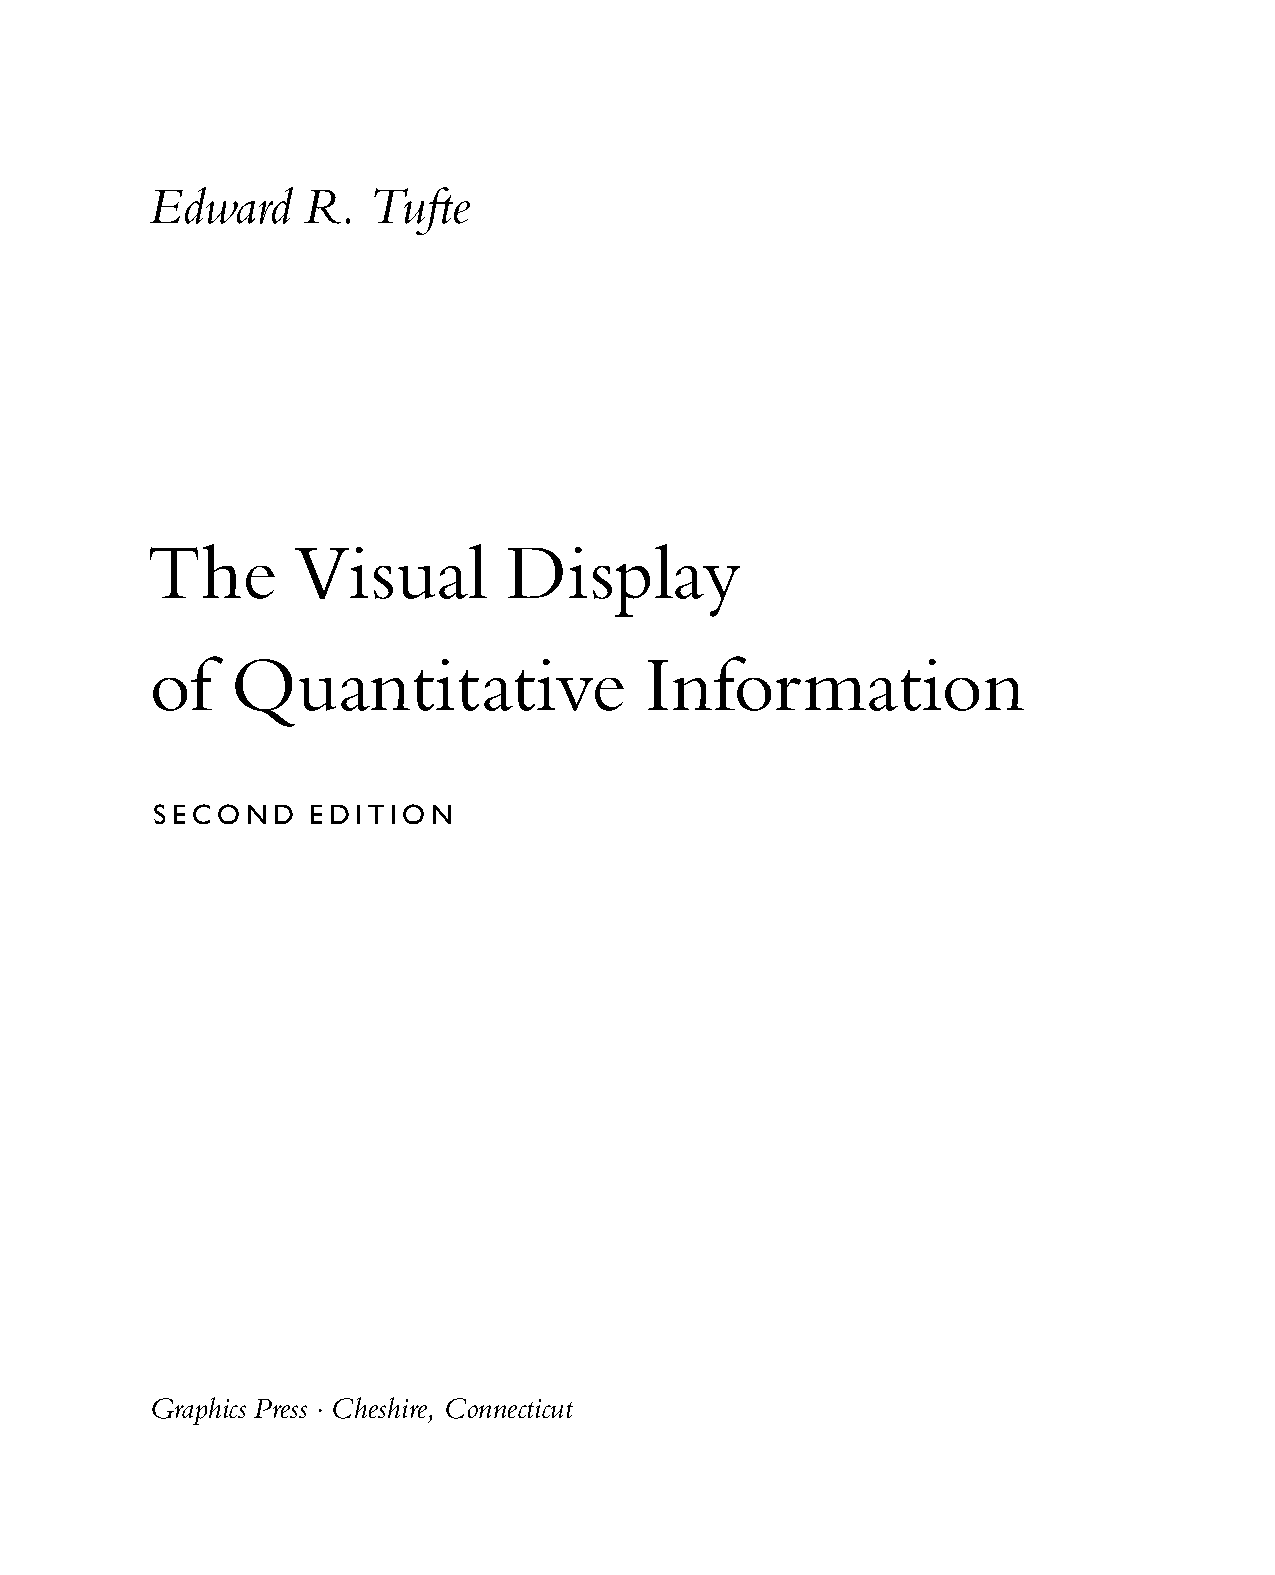
\includegraphics[width=0.45\linewidth]{graphics/vdqi-title.pdf}}
\hfill
\fbox{
\includegraphics[width=0.45\linewidth]{graphics/ei-title.pdf}}
\\\vspace{\baselineskip}
\fbox{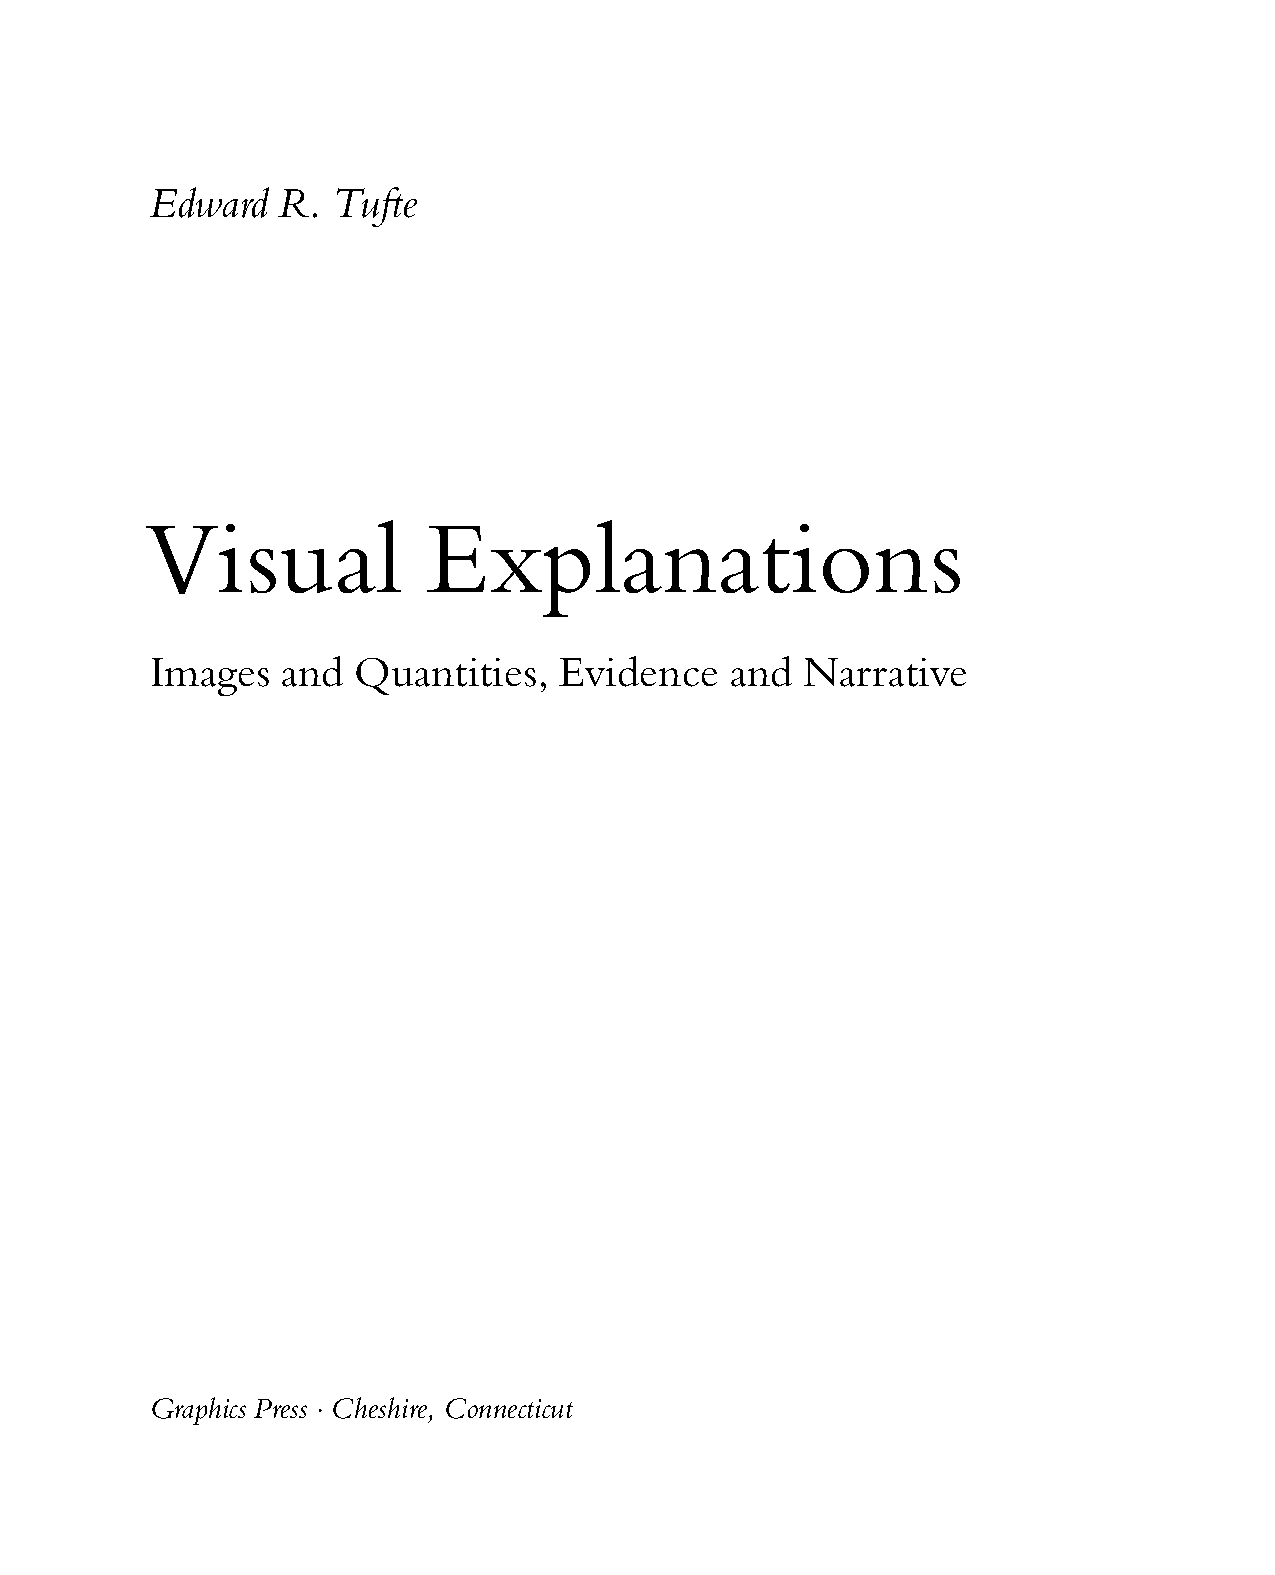
\includegraphics[width=0.45\linewidth]{graphics/ve-title.pdf}}
\hfill
\fbox{
\includegraphics[width=0.45\linewidth]{graphics/be-title.pdf}}
\end{figure*}

\newthought{The tables of contents} in Tufte's books give us our first
glimpse of the structure of the main matter.  \VDQI is split into two
parts, each containing some number of chapters.  His other three books only
contain chapters---they're not broken into parts.

\begin{figure*}[p]\index{table of contents}
\fbox{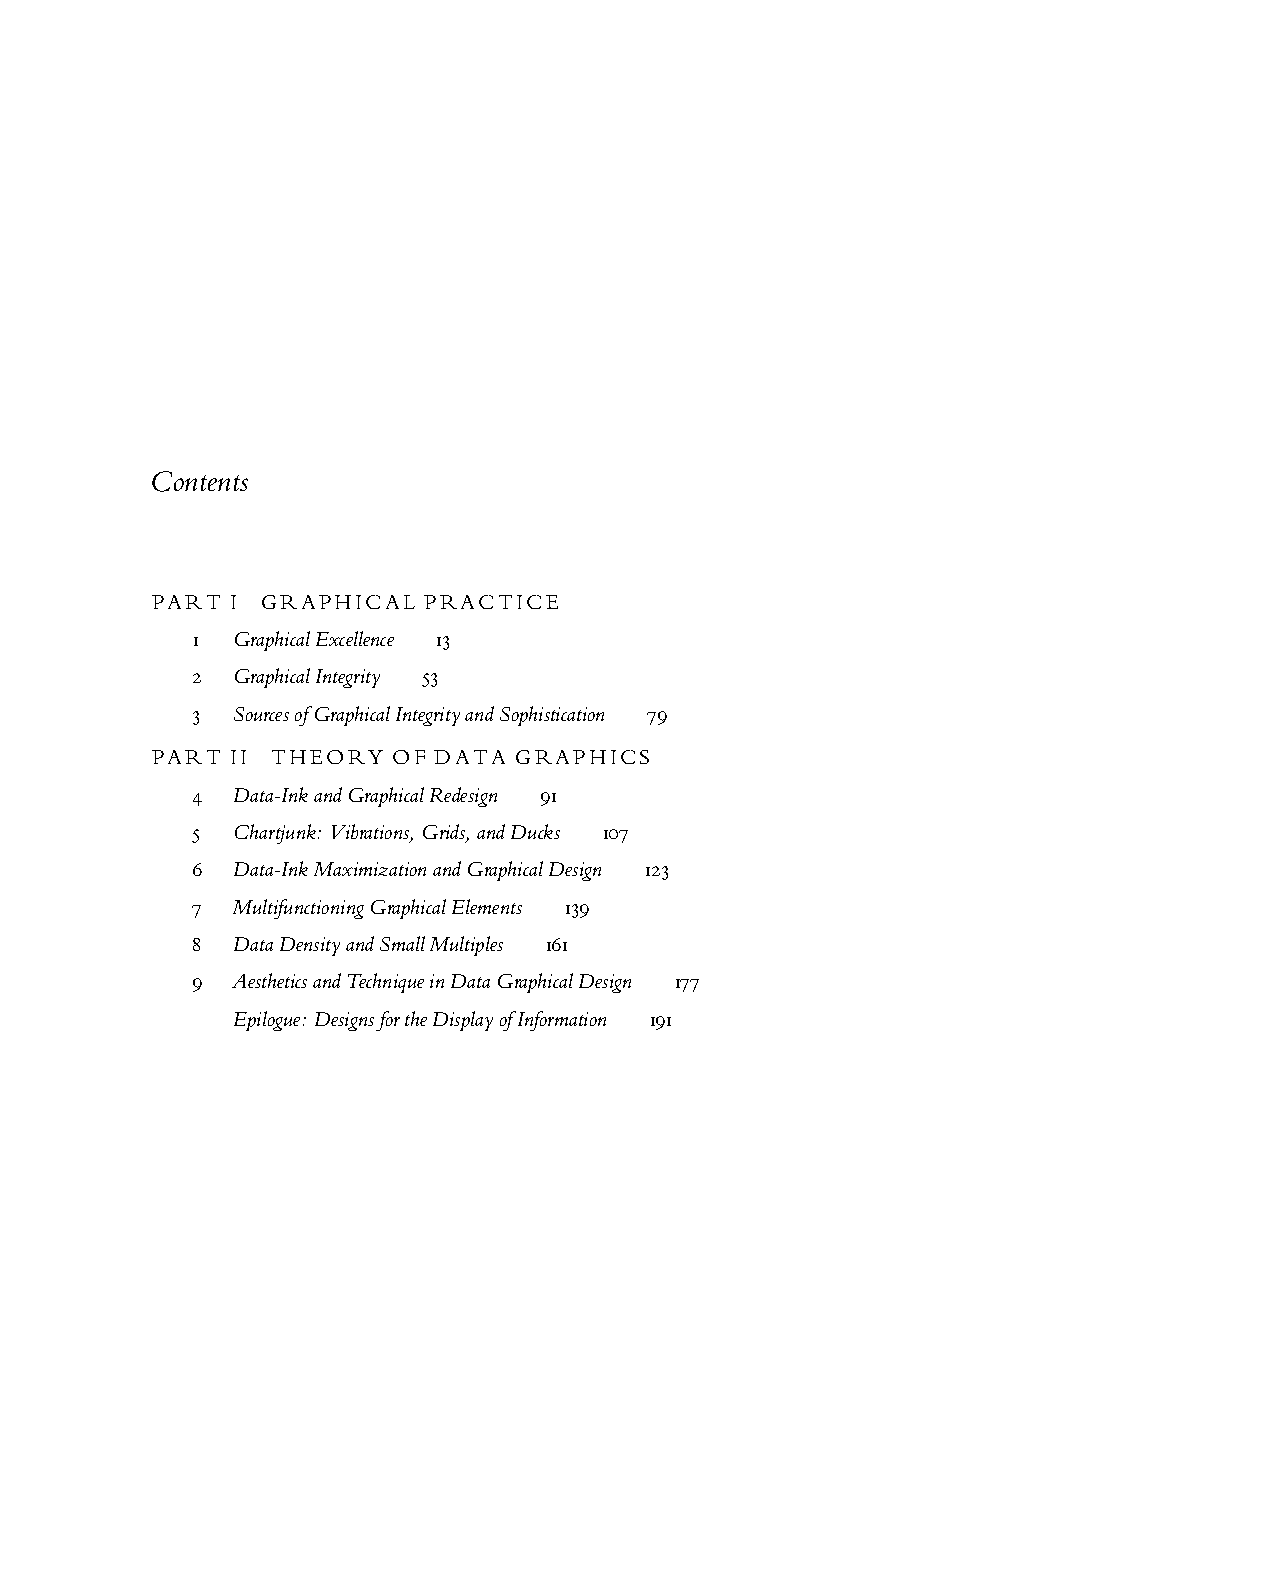
\includegraphics[width=0.45\linewidth]{graphics/vdqi-contents.pdf}}
\hfill
\fbox{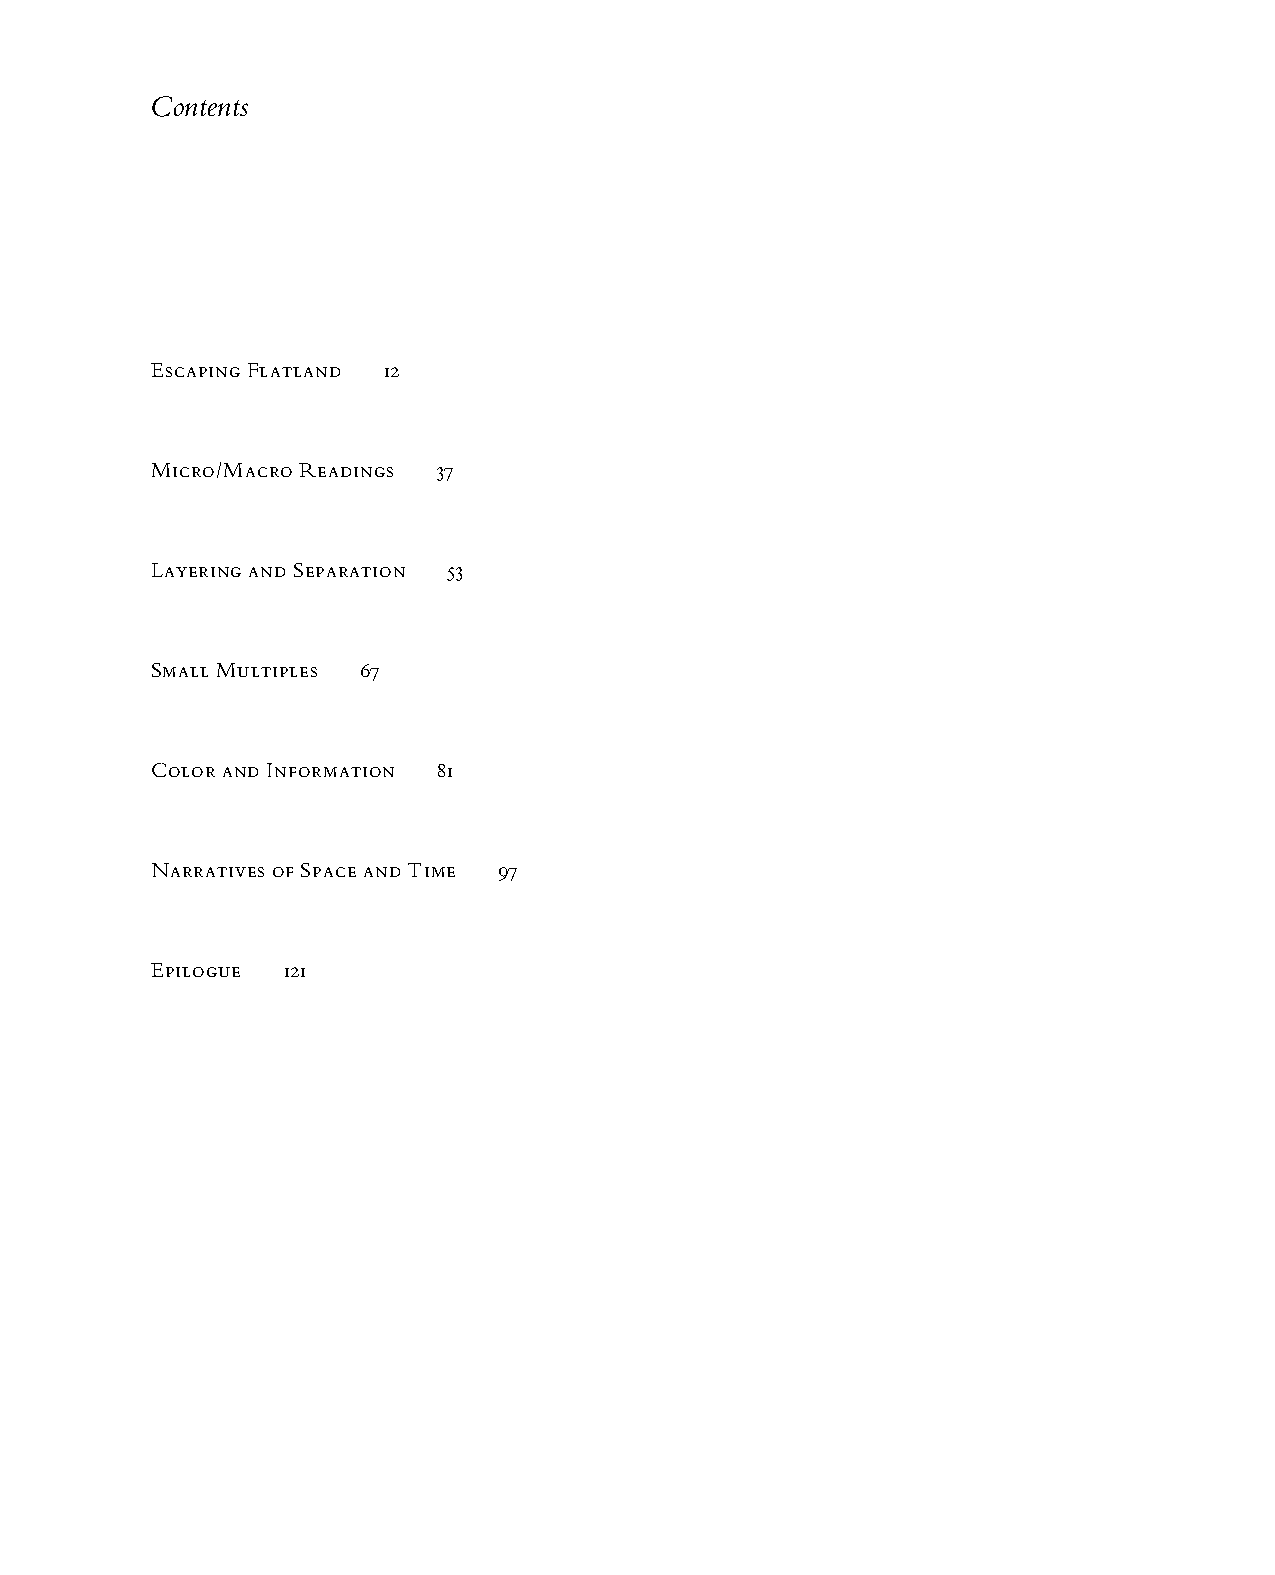
\includegraphics[width=0.45\linewidth]{graphics/ei-contents.pdf}}
\\\vspace{\baselineskip}
\fbox{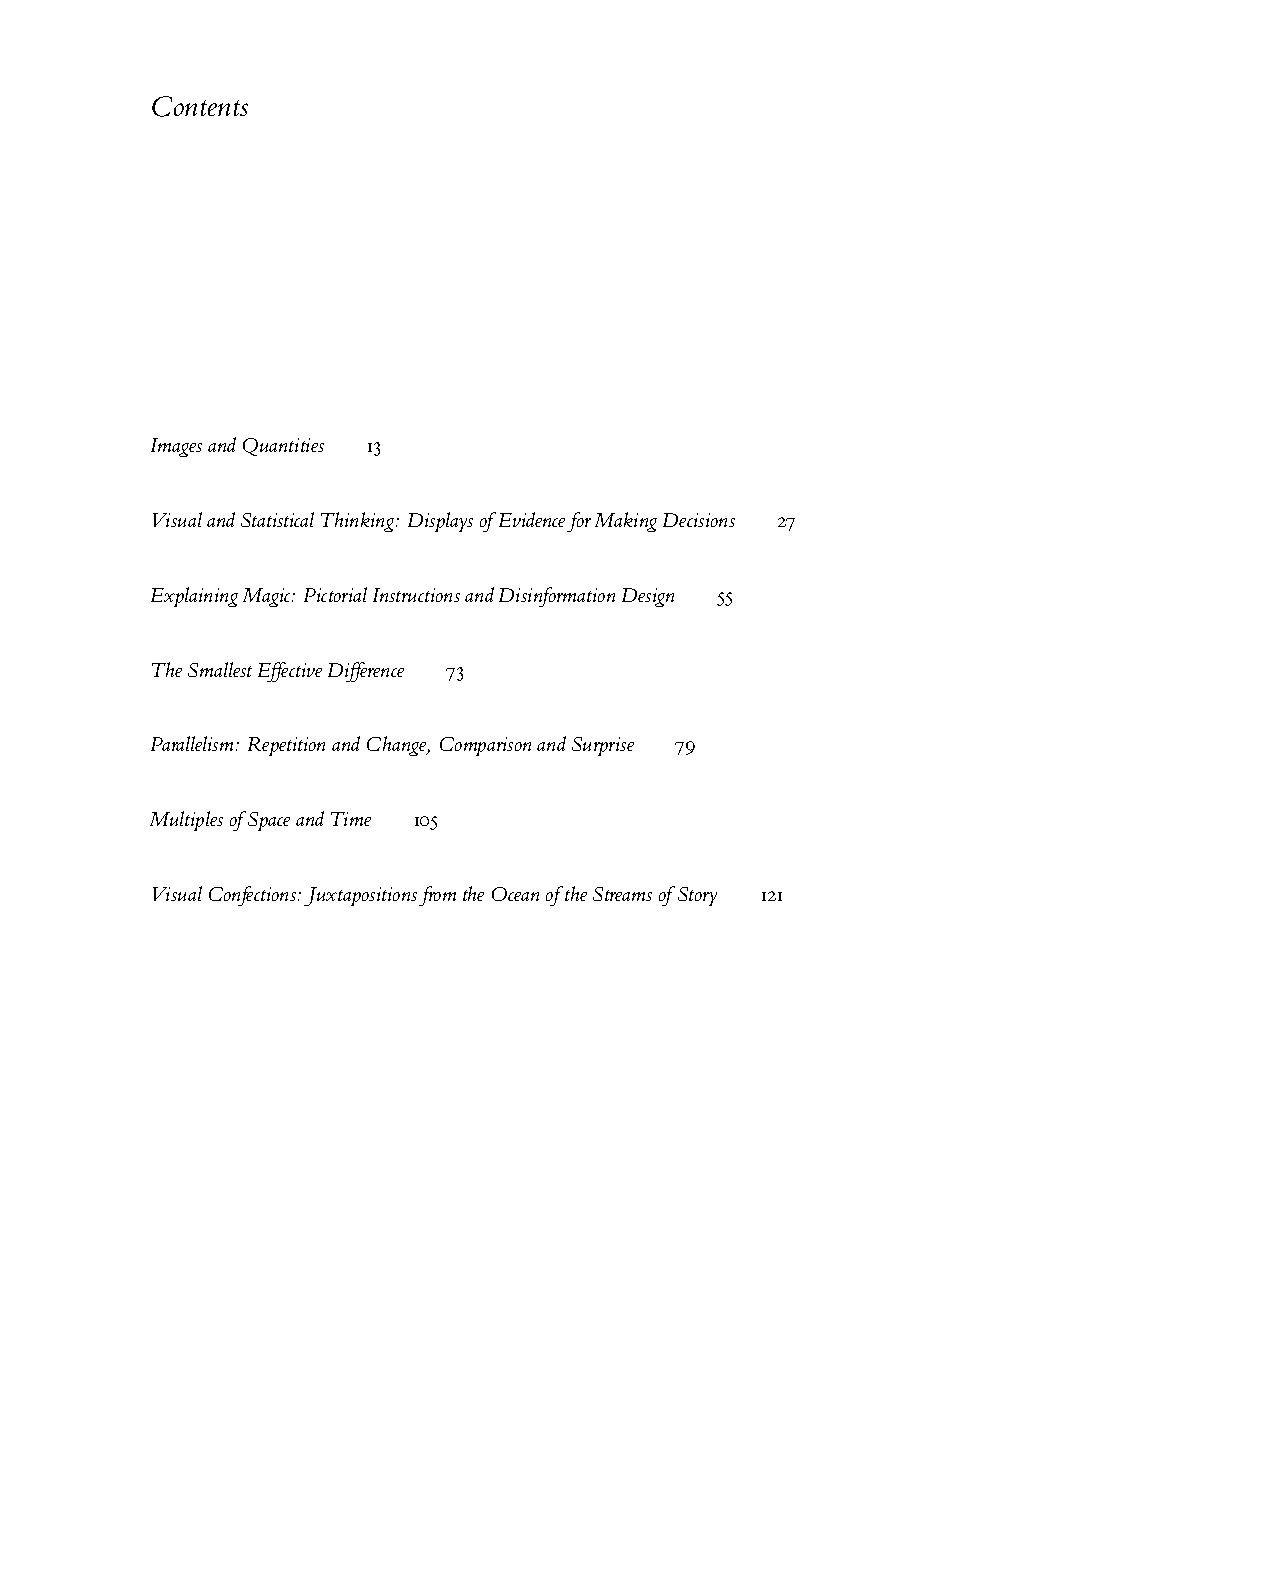
\includegraphics[width=0.45\linewidth]{graphics/ve-contents.pdf}}
\hfill
\fbox{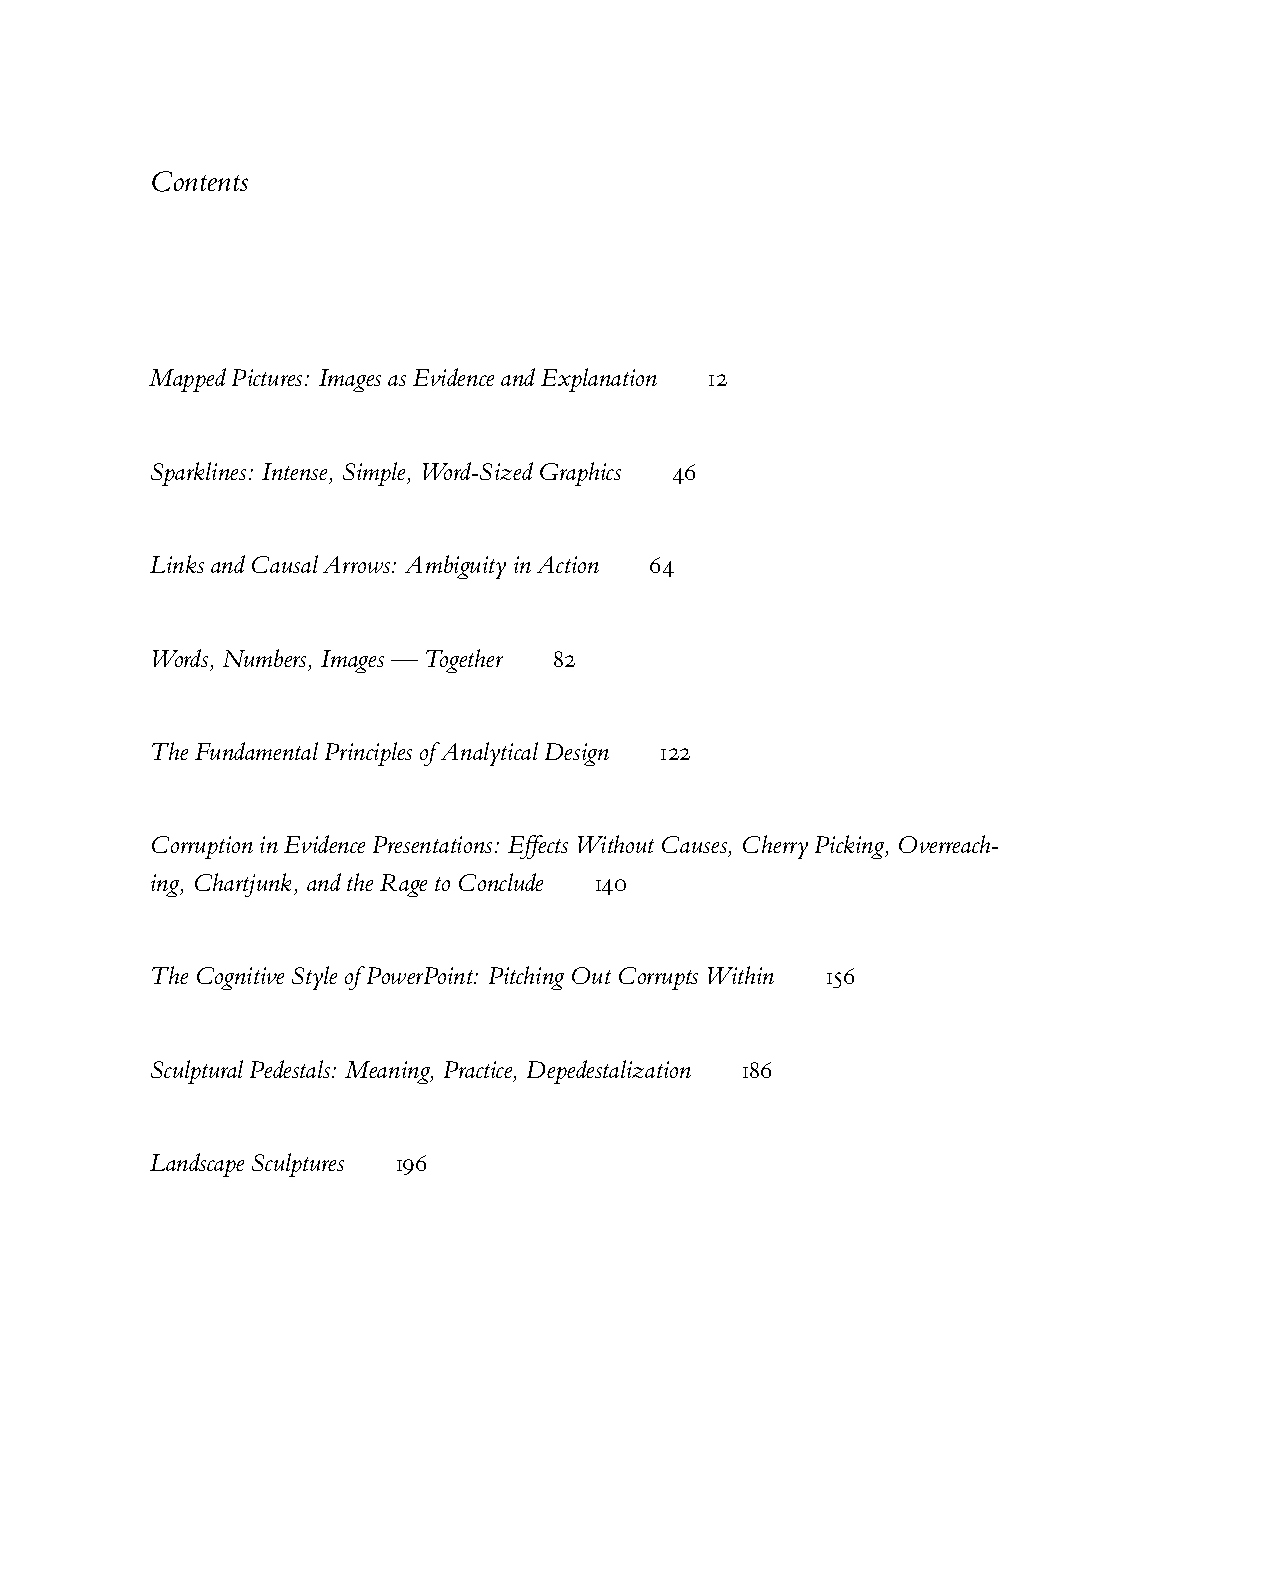
\includegraphics[width=0.45\linewidth]{graphics/be-contents.pdf}}
\end{figure*}


\section{Typefaces}\label{sec:typefaces1}\index{typefaces}
\index{fonts|see{typefaces}}

Tufte's books primarily use two typefaces: Bembo and Gill Sans.  Bembo is used
for the headings and body text, while Gill Sans is used for the title page and
opening epigraphs in \BE.

Since neither Bembo nor Gill Sans are available in default \LaTeX{}
installations, the \TL document classes default to using Palatino and
Helvetica, respectively.  In addition, the Bera Mono typeface is used for
\texttt{monospaced} type.

The following font sizes are defined by the \TL classes:

\begin{table}[h]\index{typefaces!sizes}
  \footnotesize%
  \begin{center}
    \begin{tabular}{lccl}
      \toprule
      \LaTeX{} size & Font size & Leading & Used for \\
      \midrule
      \verb+\tiny+         &  5 &  6 & sidenote numbers \\
      \verb+\scriptsize+   &  7 &  8 & \na \\
      \verb+\footnotesize+ &  8 & 10 & sidenotes, captions \\
      \verb+\small+        &  9 & 12 & quote, quotation, and verse environments \\
      \verb+\normalsize+   & 10 & 14 & body text \\
      \verb+\large+        & 11 & 15 & \textsc{b}-heads \\
      \verb+\Large+        & 12 & 16 & \textsc{a}-heads, \textsc{toc} entries, author, date \\
      \verb+\LARGE+        & 14 & 18 & handout title \\
      \verb+\huge+         & 20 & 30 & chapter heads \\
      \verb+\Huge+         & 24 & 36 & part titles \\
      \bottomrule
    \end{tabular}
  \end{center}
  \caption{A list of \LaTeX{} font sizes as defined by the \TL document classes.}
  \label{tab:font-sizes}
\end{table}

\section{Headings}\label{sec:headings1}\index{headings}

Tufte's books include the following heading levels: parts,
chapters,\sidenote{Parts and chapters are defined for the \texttt{tufte-book}
class only.}  sections, subsections, and paragraphs.  Not defined by default
are: sub-subsections and subparagraphs.

\begin{table}[h]
  \begin{center}
    \footnotesize%
    \begin{tabular}{lcr}
      \toprule
      Heading & Style & Size \\
      \midrule
      Part & roman & \measure{24}{36}{40} \\
      Chapter & italic & \measure{20}{30}{40} \\
      Section & italic & \measure{12}{16}{26} \\
      Subsection & italic & \measure{11}{15}{26} \\
      Paragraph & italic & 10/14 \\
      \bottomrule
    \end{tabular}
  \end{center}
  \caption{Heading styles used in \BE.}
  \label{tab:heading-styles}
\end{table}

\paragraph{Paragraph} Paragraph headings (as shown here) are introduced by
italicized text and separated from the main paragraph by a bit of space.

\section{Environments}

The following characteristics define the various environments:


\begin{table}[h]
  \begin{center}
    \footnotesize%
    \begin{tabular}{lcl}
      \toprule
      Environment & Font size & Notes \\
      \midrule
      Body text & \measure{10}{14}{26} & \\
      Block quote & \measure{9}{12}{24} & Block indent (left and right) by \unit[1]{pc} \\
      Sidenotes & \measure{8}{10}{12} & Sidenote number is set inline, followed by word space \\
      Captions & \measure{8}{10}{12} &  \\
      \bottomrule
    \end{tabular}
  \end{center}
  \caption{Environment styles used in \BE.}
  \label{tab:environment-styles}
\end{table}


\chapter[On the Use of the tufte-book Document Class]{On the Use of the \texttt{tufte-book} Document Class}
\label{ch:tufte-book}

The \TL document classes define a style similar to the
style Edward Tufte uses in his books and handouts.  Tufte's style is known
for its extensive use of sidenotes, tight integration of graphics with
text, and well-set typography.  This document aims to be at once a
demonstration of the features of the \TL document classes
and a style guide to their use.

\section{Классификация ОЭП}\label{sec:page-layout}
\subsection{Headings}\label{sec:headings}\index{headings}
This style provides \textsc{a}- and \textsc{b}-heads (that is,
\Verb|\section| and \Verb|\subsection|), demonstrated above.

If you need more than two levels of section headings, you'll have to define
them yourself at the moment; there are no pre-defined styles for anything below
a \Verb|\subsection|.  As Bringhurst points out in \textit{The Elements of
Typographic Style},\cite{Bringhurst2005} you should ``use as many levels of
headings as you need: no more, and no fewer.''

The \TL classes will emit an error if you try to use
\linebreak\Verb|\subsubsection| and smaller headings.

% let's start a new thought -- a new section
\newthought{In his later books},\cite{Tufte2006} Tufte
starts each section with a bit of vertical space, a non-indented paragraph,
and sets the first few words of the sentence in \textsc{small caps}.  To
accomplish this using this style, use the \doccmddef{newthought} command:
\begin{docspec}
  \doccmd{newthought}\{In his later books\}, Tufte starts\ldots
\end{docspec}


\section{Sidenotes}\label{sec:sidenotes}
One of the most prominent and distinctive features of this style is the
extensive use of sidenotes.  There is a wide margin to provide ample room
for sidenotes and small figures.  Any \doccmd{footnote}s will automatically
be converted to sidenotes.\footnote{This is a sidenote that was entered
using the \texttt{\textbackslash footnote} command.}  If you'd like to place ancillary
information in the margin without the sidenote mark (the superscript
number), you can use the \doccmd{marginnote} command.

The specification of the \doccmddef{sidenote} command is:
\begin{docspec}
  \doccmd{sidenote}[\docopt{number}][\docopt{offset}]\{\docarg{Sidenote text.}\}
\end{docspec}

Both the \docopt{number} and \docopt{offset} arguments are optional.  If you
provide a \docopt{number} argument, \marginnote{This is a
margin note.  Notice that there isn't a number preceding the note, and
there is no number in the main text where this note was written.} then that number will be used as the
sidenote number.  It will change of the number of the current sidenote only and
will not affect the numbering sequence of subsequent sidenotes.

Sometimes a sidenote may run over the top of other text or graphics in the
margin space.  If this happens, you can adjust the vertical position of the
sidenote by providing a dimension in the \docopt{offset} argument.  Some
examples of valid dimensions are:
\begin{docspec}
  \ttfamily 1.0in \qquad 2.54cm \qquad 254mm \qquad 6\Verb|\baselineskip|
\end{docspec}
If the dimension is positive it will push the sidenote down the page; if the
dimension is negative, it will move the sidenote up the page.

While both the \docopt{number} and \docopt{offset} arguments are optional, they
must be provided in order.  To adjust the vertical position of the sidenote
while leaving the sidenote number alone, use the following syntax:
\begin{docspec}
  \doccmd{sidenote}[][\docopt{offset}]\{\docarg{Sidenote text.}\}
\end{docspec}
The empty brackets tell the \Verb|\sidenote| command to use the default
sidenote number.

If you \emph{only} want to change the sidenote number, however, you may
completely omit the \docopt{offset} argument:
\begin{docspec}
  \doccmd{sidenote}[\docopt{number}]\{\docarg{Sidenote text.}\}
\end{docspec}

The \doccmddef{marginnote} command has a similar \docarg{offset} argument:
\begin{docspec}
  \doccmd{marginnote}[\docopt{offset}]\{\docarg{Margin note text.}\}
\end{docspec}

\section{References}
References are placed alongside their citations as sidenotes,
as well.  This can be accomplished using the normal \doccmddef{cite}
command.\sidenote{The first paragraph of this document includes a citation.}

The complete list of references may also be printed automatically by using
the \doccmddef{bibliography} command.  (See the end of this document for an
example.)  If you do not want to print a bibliography at the end of your
document, use the \doccmddef{nobibliography} command in its place.  

To enter multiple citations at one location,\cite[-3\baselineskip]{Tufte2006,Tufte1990} you can
provide a list of keys separated by commas and the same optional vertical
offset argument: \Verb|\cite{Tufte2006,Tufte1990}|.  
\begin{docspec}
  \doccmd{cite}[\docopt{offset}]\{\docarg{bibkey1,bibkey2,\ldots}\}
\end{docspec}

\section{Figures and Tables}\label{sec:figures-and-tables}
Images and graphics play an integral role in Tufte's work.
In addition to the standard \docenvdef{figure} and \docenvdef{tabular} environments,
this style provides special figure and table environments for full-width
floats.

Full page--width figures and tables may be placed in \docenvdef{figure*} or
\docenvdef{table*} environments.  To place figures or tables in the margin,
use the \docenvdef{marginfigure} or \docenvdef{margintable} environments as follows
(see figure~\ref{fig:marginfig}):

\begin{marginfigure}%
  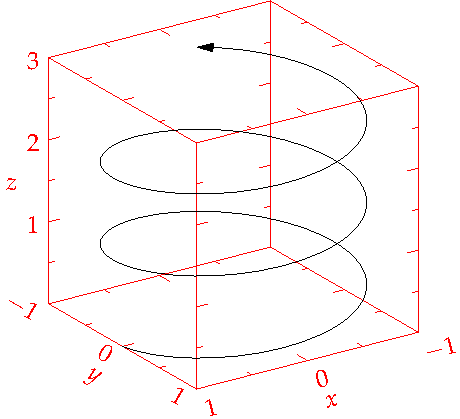
\includegraphics[width=\linewidth]{helix}
  \caption{This is a margin figure.  The helix is defined by 
    $x = \cos(2\pi z)$, $y = \sin(2\pi z)$, and $z = [0, 2.7]$.  The figure was
    drawn using Asymptote (\url{http://asymptote.sf.net/}).}
  \label{fig:marginfig}
\end{marginfigure}

\begin{docspec}
\textbackslash begin\{marginfigure\}\\
  \qquad\textbackslash includegraphics\{helix\}\\
  \qquad\textbackslash caption\{This is a margin figure.\}\\
  \qquad\textbackslash label\{fig:marginfig\}\\
\textbackslash end\{marginfigure\}\\
\end{docspec}

The \docenv{marginfigure} and \docenv{margintable} environments accept an optional parameter \docopt{offset} that adjusts the vertical position of the figure or table.  See the ``\nameref{sec:sidenotes}'' section above for examples.  The specifications are:
\begin{docspec}
  \textbackslash{begin\{marginfigure\}[\docopt{offset}]}\\
  \qquad\ldots\\
  \textbackslash{end\{marginfigure\}}\\
  \mbox{}\\
  \textbackslash{begin\{margintable\}[\docopt{offset}]}\\
  \qquad\ldots\\
  \textbackslash{end\{margintable\}}\\
\end{docspec}

Figure~\ref{fig:fullfig} is an example of the \docenv{figure*}
environment and figure~\ref{fig:textfig} is an example of the normal
\docenv{figure} environment.

\begin{figure*}[h]
  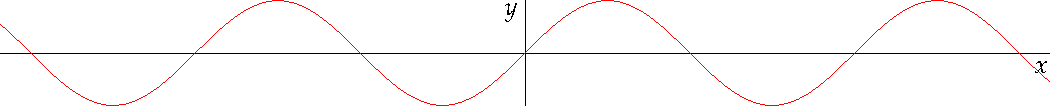
\includegraphics[width=\linewidth]{sine.pdf}%
  \caption{This graph shows $y = \sin x$ from about $x = [-10, 10]$.
  \emph{Notice that this figure takes up the full page width.}}%
  \label{fig:fullfig}%
\end{figure*}

\begin{figure}
  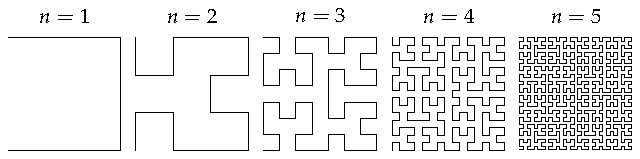
\includegraphics{hilbertcurves.pdf}
%  \checkparity This is an \pageparity\ page.%
  \caption[Hilbert curves of various degrees $n$.][6pt]{Hilbert curves of various degrees $n$. \emph{Notice that this figure only takes up the main textblock width.}}
  \label{fig:textfig}
  %\zsavepos{pos:textfig}
\end{figure}

As with sidenotes and marginnotes, a caption may sometimes require vertical
adjustment. The \doccmddef{caption} command now takes a second optional
argument that enables you to do this by providing a dimension \docopt{offset}.
You may specify the caption in any one of the following forms:
\begin{docspec}
  \doccmd{caption}\{\docarg{long caption}\}\\
  \doccmd{caption}[\docarg{short caption}]\{\docarg{long caption}\}\\
  \doccmd{caption}[][\docopt{offset}]\{\docarg{long caption}\}\\
  \doccmd{caption}[\docarg{short caption}][\docopt{offset}]%
                  \{\docarg{long caption}\}
\end{docspec}
A positive \docopt{offset} will push the caption down the page. The short
caption, if provided, is what appears in the list of figures/tables, otherwise
the ``long'' caption appears there. Note that although the arguments
\docopt{short caption} and \docopt{offset} are both optional, they must be
provided in order. Thus, to specify an \docopt{offset} without specifying a
\docopt{short caption}, you must include the first set of empty brackets
\Verb|[]|, which tell \doccmd{caption} to use the default ``long'' caption. As
an example, the caption to figure~\ref{fig:textfig} above was given in the form
\begin{docspec}
  \doccmd{caption}[Hilbert curves...][6pt]\{Hilbert curves...\}
\end{docspec}

Table~\ref{tab:normaltab} shows table created with the \docpkg{booktabs}
package.  Notice the lack of vertical rules---they serve only to clutter
the table's data.

\begin{table}[ht]
  \centering
  \fontfamily{ppl}\selectfont
  \begin{tabular}{ll}
    \toprule
    Margin & Length \\
    \midrule
    Paper width & \unit[8\nicefrac{1}{2}]{inches} \\
    Paper height & \unit[11]{inches} \\
    Textblock width & \unit[6\nicefrac{1}{2}]{inches} \\
    Textblock/sidenote gutter & \unit[\nicefrac{3}{8}]{inches} \\
    Sidenote width & \unit[2]{inches} \\
    \bottomrule
  \end{tabular}
  \caption{Here are the dimensions of the various margins used in the Tufte-handout class.}
  \label{tab:normaltab}
  %\zsavepos{pos:normaltab}
\end{table}

\newthought{Occasionally} \LaTeX{} will generate an error message:\label{err:too-many-floats}
\begin{docspec}
  Error: Too many unprocessed floats
\end{docspec}
\LaTeX{} tries to place floats in the best position on the page.  Until it's
finished composing the page, however, it won't know where those positions are.
If you have a lot of floats on a page (including sidenotes, margin notes,
figures, tables, etc.), \LaTeX{} may run out of ``slots'' to keep track of them
and will generate the above error.

\LaTeX{} initially allocates 18 slots for storing floats.  To work around this
limitation, the \TL document classes provide a \doccmddef{morefloats} command
that will reserve more slots.

The first time \doccmd{morefloats} is called, it allocates an additional 34
slots.  The second time \doccmd{morefloats} is called, it allocates another 26
slots.

The \doccmd{morefloats} command may only be used two times.  Calling it a
third time will generate an error message.  (This is because we can't safely
allocate many more floats or \LaTeX{} will run out of memory.)

If, after using the \doccmd{morefloats} command twice, you continue to get the
\texttt{Too many unprocessed floats} error, there are a couple things you can
do.

The \doccmddef{FloatBarrier} command will immediately process all the floats
before typesetting more material.  Since \doccmd{FloatBarrier} will start a new
paragraph, you should place this command at the beginning or end of a
paragraph.

The \doccmddef{clearpage} command will also process the floats before
continuing, but instead of starting a new paragraph, it will start a new page.

You can also try moving your floats around a bit: move a figure or table to the
next page or reduce the number of sidenotes.  (Each sidenote actually uses
\emph{two} slots.)

After the floats have placed, \LaTeX{} will mark those slots as unused so they
are available for the next page to be composed.

\section{Captions}
You may notice that the captions are sometimes misaligned.
Due to the way \LaTeX's float mechanism works, we can't know for sure where it
decided to put a float. Therefore, the \TL document classes provide commands to
override the caption position.

\paragraph{Vertical alignment} To override the vertical alignment, use the
\doccmd{setfloatalignment} command inside the float environment.  For
example:

\begin{fullwidth}
\begin{docspec}
  \textbackslash begin\{figure\}[btp]\\
  \qquad \textbackslash includegraphics\{sinewave\}\\
  \qquad \textbackslash caption\{This is an example of a sine wave.\}\\
  \qquad \textbackslash label\{fig:sinewave\}\\
  \qquad \hlred{\textbackslash setfloatalignment\{b\}\% forces caption to be bottom-aligned}\\
  \textbackslash end\{figure\}
\end{docspec}
\end{fullwidth}

\noindent The syntax of the \doccmddef{setfloatalignment} command is:

\begin{docspec}
  \doccmd{setfloatalignment}\{\docopt{pos}\}
\end{docspec}

\noindent where \docopt{pos} can be either \texttt{b} for bottom-aligned
captions, or \texttt{t} for top-aligned captions.

\paragraph{Horizontal alignment}\label{par:overriding-horizontal}
To override the horizontal alignment, use either the \doccmd{forceversofloat}
or the \doccmd{forcerectofloat} command inside of the float environment.  For
example:

\begin{fullwidth}
\begin{docspec}
  \textbackslash begin\{figure\}[btp]\\
  \qquad \textbackslash includegraphics\{sinewave\}\\
  \qquad \textbackslash caption\{This is an example of a sine wave.\}\\
  \qquad \textbackslash label\{fig:sinewave\}\\
  \qquad \hlred{\textbackslash forceversofloat\% forces caption to be set to the left of the float}\\
  \textbackslash end\{figure\}
\end{docspec}
\end{fullwidth}

The \doccmddef{forceversofloat} command causes the algorithm to assume the
float has been placed on a verso page---that is, a page on the left side of a
two-page spread.  Conversely, the \doccmddef{forcerectofloat} command causes
the algorithm to assume the float has been placed on a recto page---that is, a
page on the right side of a two-page spread.


\section{Full-width text blocks}

In addition to the new float types, there is a \docenvdef{fullwidth}
environment that stretches across the main text block and the sidenotes
area.

\begin{Verbatim}
\begin{fullwidth}
Lorem ipsum dolor sit amet...
\end{fullwidth}
\end{Verbatim}

\begin{fullwidth}
\small\itshape\lipsum[1]
\end{fullwidth}

\section{Typography}\label{sec:typography}

\subsection{Typefaces}\label{sec:typefaces}\index{typefaces}
If the Palatino, \textsf{Helvetica}, and \texttt{Bera Mono} typefaces are installed, this style
will use them automatically.  Otherwise, we'll fall back on the Computer Modern
typefaces.

\subsection{Letterspacing}\label{sec:letterspacing}
This document class includes two new commands and some improvements on
existing commands for letterspacing.

When setting strings of \allcaps{ALL CAPS} or \smallcaps{small caps}, the
letter\-spacing---that is, the spacing between the letters---should be
increased slightly.\cite{Bringhurst2005}  The \doccmddef{allcaps} command has proper letterspacing for
strings of \allcaps{FULL CAPITAL LETTERS}, and the \doccmddef{smallcaps} command
has letterspacing for \smallcaps{small capital letters}.  These commands
will also automatically convert the case of the text to upper- or
lowercase, respectively.

The \doccmddef{textsc} command has also been redefined to include
letterspacing.  The case of the \doccmd{textsc} argument is left as is,
however.  This allows one to use both uppercase and lowercase letters:
\textsc{The Initial Letters Of The Words In This Sentence Are Capitalized.}



\section{Document Class Options}\label{sec:options}

\index{class options|(}
The \doccls{tufte-book} class is based on the \LaTeX\ \doccls{book}
document class.  Therefore, you can pass any of the typical book
options.  There are a few options that are specific to the
\doccls{tufte-book} document class, however.

The \docclsoptdef{a4paper} option will set the paper size to \smallcaps{A4} instead of
the default \smallcaps{US} letter size.

The \docclsoptdef{sfsidenotes} option will set the sidenotes and title block in a 
\textsf{sans serif} typeface instead of the default roman.

The \docclsoptdef{twoside} option will modify the running heads so that the page
number is printed on the outside edge (as opposed to always printing the page
number on the right-side edge in \docclsoptdef{oneside} mode).  

The \docclsoptdef{symmetric} option typesets the sidenotes on the outside edge of
the page.  This is how books are traditionally printed, but is contrary to
Tufte's book design which sets the sidenotes on the right side of the page.
This option implicitly sets the \docclsopt{twoside} option.

The \docclsoptdef{justified} option sets all the text fully justified (flush left
and right).  The default is to set the text ragged right.  
The body text of Tufte's books are set ragged right.  This prevents
needless hyphenation and makes it easier to read the text in the slightly
narrower column.

The \docclsoptdef{bidi} option loads the \docpkg{bidi} package which is used with
\tXeLaTeX\ to typeset bi-directional text.  Since the \docpkg{bidi}
package needs to be loaded before the sidenotes and cite commands are defined,
it can't be loaded in the document preamble.

The \docclsoptdef{debug} option causes the \TL classes to output debug
information to the log file which is useful in troubleshooting bugs.  It will
also cause the graphics to be replaced by outlines.

The \docclsoptdef{nofonts} option prevents the \TL classes from
automatically loading the Palatino and Helvetica typefaces.  You should use
this option if you wish to load your own fonts.  If you're using \tXeLaTeX, this
option is implied (\ie, the Palatino and Helvetica fonts aren't loaded if you
use \tXeLaTeX).  

The \docclsoptdef{nols} option inhibits the letterspacing code.  The \TL\
classes try to load the appropriate letterspacing package (either pdf\TeX's
\docpkg{letterspace} package or the \docpkg{soul} package).  If you're using
\tXeLaTeX\ with \docpkg{fontenc}, however, you should configure your own
letterspacing.  

The \docclsoptdef{notitlepage} option causes \doccmd{maketitle} to generate a title
block instead of a title page.  The \doccls{book} class defaults to a title
page and the \doccls{handout} class defaults to the title block.  There is an
analogous \docclsoptdef{titlepage} option that forces \doccmd{maketitle} to
generate a full title page instead of the title block.

The \docclsoptdef{notoc} option suppresses \TL's custom table of contents
(\textsc{toc}) design.  The current \textsc{toc} design only shows unnumbered
chapter titles; it doesn't show sections or subsections.  The \docclsopt{notoc}
option will revert to \LaTeX's \textsc{toc} design.

The \docclsoptdef{nohyper} option prevents the \docpkg{hyperref} package from
being loaded.  The default is to load the \docpkg{hyperref} package and use the
\doccmd{title} and \doccmd{author} contents as metadata for the generated
\textsc{pdf}.

\index{class options|)}



\chapter[Customizing Tufte-LaTeX]{Customizing \TL}
\label{ch:customizing}

The \TL document classes are designed to closely emulate Tufte's book
design by default.  However, each document is different and you may encounter
situations where the default settings are insufficient.  This chapter explores
many of the ways you can adjust the \TL document classes to better fit
your needs.

\section{File Hooks}
\label{sec:filehooks}

\index{file hooks|(}
If you create many documents using the \TL classes, it's easier to
store your customizations in a separate file instead of copying them into the
preamble of each document.  The \TL classes provide three file hooks:
\docfilehook{tufte-common-local.tex}{common}, \docfilehook{tufte-book-local.tex}{book}, and
\docfilehook{tufte-handout-local.tex}{handout}.\sloppy

\begin{description}
  \item[\docfilehook{tufte-common-local.tex}{common}]
    If this file exists, it will be loaded by all of the \TL document
    classes just prior to any document-class-specific code.  If your
    customizations or code should be included in both the book and handout
    classes, use this file hook.
  \item[\docfilehook{tufte-book-local.tex}{book}] 
    If this file exists, it will be loaded after all of the common and
    book-specific code has been read.  If your customizations apply only to the
    book class, use this file hook.
  \item[\docfilehook{tufte-common-handout.tex}{handout}] 
    If this file exists, it will be loaded after all of the common and
    handout-specific code has been read.  If your customizations apply only to
    the handout class, use this file hook.
\end{description}

\index{file hooks|)}

\section{Numbered Section Headings}
\label{sec:numbered-sections}
\index{headings!numbered}

While Tufte dispenses with numbered headings in his books, if you require them,
they can be anabled by changing the value of the \doccounter{secnumdepth}
counter.  From the table below, select the heading level at which numbering
should stop and set the \doccounter{secnumdepth} counter to that value.  For
example, if you want parts and chapters numbered, but don't want numbering for
sections or subsections, use the command:
\begin{docspec}
  \doccmd{setcounter}\{secnumdepth\}\{0\}
\end{docspec}

The default \doccounter{secnumdepth} for the \TL document classes is $-1$.

\begin{table}
  \footnotesize
  \begin{center}
    \begin{tabular}{lr}
      \toprule
      Heading level & Value \\
      \midrule
      Part (in \doccls{tufte-book}) & $-1$ \\
      Part (in \doccls{tufte-handout}) & $0$ \\
      Chapter (only in \doccls{tufte-book}) & $0$ \\
      Section & $1$ \\
      Subsection & $2$ \\
      Subsubsection & $3$ \\
      Paragraph & $4$ \\
      Subparagraph & $5$ \\
      \bottomrule
    \end{tabular}
  \end{center}
  \caption{Heading levels used with the \texttt{secnumdepth} counter.}
\end{table}

\section{Changing the Paper Size}
\label{sec:paper-size}

The \TL classes currently only provide three paper sizes: \textsc{a4},
\textsc{b5}, and \textsc{us} letter.  To specify a different paper size (and/or
margins), use the \doccmd[geometry]{geometry} command in the preamble of your
document (or one of the file hooks).  The full documentation of the
\doccmd{geometry} command may be found in the \docpkg{geometry} package
documentation.\cite{pkg-geometry}


\section{Customizing Marginal Material}
\label{sec:marginal-material}

Marginal material includes sidenotes, citations, margin notes, and captions.
Normally, the justification of the marginal material follows the justification
of the body text.  If you specify the \docclsopt{justified} document class
option, all of the margin material will be fully justified as well.  If you
don't specify the \docclsopt{justified} option, then the marginal material will
be set ragged right.

You can set the justification of the marginal material separately from the body
text using the following document class options: \docclsopt{sidenote},
\docclsopt{marginnote}, \docclsopt{caption}, \docclsopt{citation}, and
\docclsopt{marginals}.  Each option refers to its obviously corresponding
marginal material type.  The \docclsopt{marginals} option simultaneously sets
the justification on all four marginal material types.

Each of the document class options takes one of five justification types:
\begin{description}
  \item[\docclsopt{justified}] Fully justifies the text (sets it flush left and
    right).
  \item[\docclsopt{raggedleft}] Sets the text ragged left, regardless of which
    page it falls on.
  \item[\docclsopt{raggedright}] Sets the text ragged right, regardless of
    which page it falls on.
  \item[\doccls{raggedouter}] Sets the text ragged left if it falls on the
    left-hand (verso) page of the spread and otherwise sets it ragged right.
    This is useful in conjunction with the \docclsopt{symmetric} document class
    option.
  \item[\docclsopt{auto}] If the \docclsopt{justified} document class option
    was specified, then set the text fully justified; otherwise the text is set
    ragged right.  This is the default justification option if one is not
    explicitly specified.
\end{description}

\noindent For example, 
\begin{docspec}
  \doccmdnoindex{documentclass}[symmetric,justified,marginals=raggedouter]\{tufte-book\}
\end{docspec}
will set the body text of the document to be fully justified and all of the
margin material (sidenotes, margin notes, captions, and citations) to be flush
against the body text with ragged outer edges.

\newthought{The font and style} of the marginal material may also be modified using the following commands:

\begin{docspec}
  \doccmd{setsidenotefont}\{\docopt{font commands}\}\\
  \doccmd{setcaptionfont}\{\docopt{font commands}\}\\
  \doccmd{setmarginnotefont}\{\docopt{font commands}\}\\
  \doccmd{setcitationfont}\{\docopt{font commands}\}
\end{docspec}

The \doccmddef{setsidenotefont} sets the font and style for sidenotes, the
\doccmddef{setcaptionfont} for captions, the \doccmddef{setmarginnotefont} for
margin notes, and the \doccmddef{setcitationfont} for citations.  The
\docopt{font commands} can contain font size changes (e.g.,
\doccmdnoindex{footnotesize}, \doccmdnoindex{Huge}, etc.), font style changes (e.g.,
\doccmdnoindex{sffamily}, \doccmdnoindex{ttfamily}, \doccmdnoindex{itshape}, etc.), color changes (e.g.,
\doccmdnoindex{color}\texttt{\{blue\}}), and many other adjustments.

If, for example, you wanted the captions to be set in italic sans serif, you could use:
\begin{docspec}
  \doccmd{setcaptionfont}\{\doccmdnoindex{itshape}\doccmdnoindex{sffamily}\}
\end{docspec}

\chapter{Compatibility Issues}
\label{ch:compatibility}

When switching an existing document from one document class to a \TL document class, a few changes to the document may have to be made.

\section{Converting from \doccls{article} to \doccls{tufte-handout}}

The following \doccls{article} class options are unsupported: \docclsopt{10pt}, \docclsopt{11pt}, \docclsopt{12pt}, \docclsopt{a5paper}, \docclsopt{b5paper}, \docclsopt{executivepaper}, \docclsopt{legalpaper}, \docclsopt{landscape}, \docclsopt{onecolumn}, and \doccls{twocolumn}.

The following headings are not supported: \doccmd{subsubsection} and \doccmd{subparagraph}.

\section{Converting from \doccls{book} to \doccls{tufte-book}}

The following \doccls{report} class options are unsupported: \docclsopt{10pt}, \docclsopt{11pt}, \docclsopt{12pt}, \docclsopt{a5paper}, \docclsopt{b5paper}, \docclsopt{executivepaper}, \docclsopt{legalpaper}, \docclsopt{landscape}, \docclsopt{onecolumn}, and \doccls{twocolumn}.

The following headings are not supported: \doccmd{subsubsection} and \doccmd{subparagraph}.



\chapter{Troubleshooting and Support}
\label{ch:troubleshooting}

\section{\TL Website}\label{sec:website}
The website for the \TL packages is located at
\url{http://code.google.com/p/tufte-latex/}.  On our website, you'll find
links to our \smallcaps{svn} repository, mailing lists, bug tracker, and documentation.

\section{\TL Mailing Lists}\label{sec:mailing-lists}
There are two mailing lists for the \TL project:

\paragraph{Discussion list}
The \texttt{tufte-latex} discussion list is for asking questions, getting
assistance with problems, and help with troubleshooting.  Release announcements
are also posted to this list.  You can subscribe to the \texttt{tufte-latex}
discussion list at \url{http://groups.google.com/group/tufte-latex}.

\paragraph{Commits list}
The \texttt{tufte-latex-commits} list is a read-only mailing list.  A message
is sent to the list any time the \TL code has been updated.  If you'd like to
keep up with the latest code developments, you may subscribe to this list.  You
can subscribe to the \texttt{tufte-latex-commits} mailing list at
\url{http://groups.google.com/group/tufte-latex-commits}.

\section{Getting Help}\label{sec:getting-help}
If you've encountered a problem with one of the \TL document classes, have a
question, or would like to report a bug, please send an email to our
mailing list or visit our website.

To help us troubleshoot the problem more quickly, please try to compile your
document using the \docclsopt{debug} class option and send the generated
\texttt{.log} file to the mailing list with a brief description of the problem.



\section{Errors, Warnings, and Informational Messages}\label{sec:tl-messages}
The following is a list of all of the errors, warnings, and other messages generated by the \TL classes and a brief description of their meanings.
\index{error messages}\index{warning messages}\index{debug messages}

% Errors
\docmsg{Error: \doccmd{subparagraph} is undefined by this class.}{%
The \doccmd{subparagraph} command is not defined in the \TL document classes.
If you'd like to use the \doccmd{subparagraph} command, you'll need to redefine
it yourself.  See the ``Headings'' section on page~\pageref{sec:headings} for a
description of the heading styles available in the \TL document classes.}

\docmsg{Error: \doccmd{subsubsection} is undefined by this class.}{%
The \doccmd{subsubsection} command is not defined in the \TL document classes.
If you'd like to use the \doccmd{subsubsection} command, you'll need to
redefine it yourself.  See the ``Headings'' section on
page~\pageref{sec:headings} for a description of the heading styles available
in the \TL document classes.}

\docmsg{Error: You may only call \doccmd{morefloats} twice. See the\par\noindent\ \ \ \ \ \ \ \ Tufte-LaTeX documentation for other workarounds.}{%
\LaTeX{} allocates 18 slots for storing floats.  The first time
\doccmd{morefloats} is called, it allocates an additional 34 slots.  The second
time \doccmd{morefloats} is called, it allocates another 26 slots.

The \doccmd{morefloats} command may only be called two times.  Calling it a
third time will generate this error message.  See
page~\pageref{err:too-many-floats} for more information.}

% Warnings
\docmsg{Warning: Option `\docopt{class option}' is not supported -{}- ignoring option.}{%
This warning appears when you've tried to use \docopt{class option} with a \TL
document class, but \docopt{class option} isn't supported by the \TL document
class.  In this situation, \docopt{class option} is ignored.}

% Info / Debug messages
\docmsg{Info: The `\docclsopt{symmetric}' option implies `\docclsopt{twoside}'}{%
You specified the \docclsopt{symmetric} document class option.  This option automatically forces the \docclsopt{twoside} option as well.  See page~\pageref{clsopt:symmetric} for more information on the \docclsopt{symmetric} class option.}


\section{Package Dependencies}\label{sec:dependencies}
The following is a list of packages that the \TL document
classes rely upon.  Packages marked with an asterisk are optional.
\begin{multicols}{2}
\begin{itemize}
  \item xifthen
  \item ifpdf*
  \item ifxetex*
  \item hyperref
  \item geometry
  \item ragged2e
  \item chngpage \emph{or} changepage
  \item paralist
  \item textcase
  \item soul*
  \item letterspace*
  \item setspace
  \item natbib \emph{and} bibentry
  \item optparams
  \item placeins
  \item mathpazo*
  \item helvet*
  \item fontenc
  \item beramono*
  \item fancyhdr
  \item xcolor
  \item textcomp
  \item titlesec
  \item titletoc
\end{itemize}
\end{multicols}




%%
% The back matter contains appendices, bibliographies, indices, glossaries, etc.







\backmatter

\bibliography{sample-handout}
\bibliographystyle{plainnat}


\printindex

\end{document}

